%====================================================
% THE GEOMETRY OF THE CURE — Academic Paper (v0.1)
% Target: PLOS Computational Biology / Nature Computational Science
%====================================================
\documentclass[11pt]{article}

% ---------- Encoding & Fonts ----------
\usepackage[T1]{fontenc}
\usepackage[utf8]{inputenc}
\usepackage[expansion=false]{microtype}
% lmodern omitted (not available in this environment)

% ---------- Page Layout ----------
\usepackage[margin=1in]{geometry}
\usepackage{setspace}
\setstretch{1.08}

% ---------- Math & Symbols ----------
\usepackage{amsmath,amssymb,amsfonts,amsthm}
\usepackage{mathtools}
\usepackage{bm}

% ---------- Graphics & Tables ----------
\usepackage{graphicx}
\usepackage{booktabs}
\usepackage{multirow}
\usepackage{array}
\usepackage{tikz}
\usepackage{pgfplots}
\pgfplotsset{compat=1.18}
\usetikzlibrary{patterns}

% ---------- Links & Refs ----------
\usepackage[hidelinks]{hyperref}
\usepackage[capitalise,nameinlink]{cleveref}

% ---------- Lists ----------
\usepackage{enumitem}
\setlist[itemize]{leftmargin=*, itemsep=2pt, topsep=2pt}
\setlist[enumerate]{leftmargin=*, itemsep=2pt, topsep=2pt}

% ---------- Theorem Environments ----------
\theoremstyle{plain}
\newtheorem{theorem}{Theorem}[section]
\newtheorem{lemma}[theorem]{Lemma}
\newtheorem{corollary}[theorem]{Corollary}
\newtheorem{proposition}[theorem]{Proposition}

\theoremstyle{definition}
\newtheorem{definition}[theorem]{Definition}
\newtheorem{remark}[theorem]{Remark}
\newtheorem{assumption}[theorem]{Assumption}

% ---------- Macros ----------
\newcommand{\mirador}{\textsc{Mirador}}
\newcommand{\Kpath}{K_{\mathrm{pathway}}}
\newcommand{\Kbarr}{K_{\mathrm{barrier}}}
\newcommand{\Kpheno}{K_{\mathrm{phenotype}}}
\newcommand{\Kres}{K_{\mathrm{reservoir}}}
\newcommand{\Kadmet}{K_{\mathrm{ADMET}}}
\newcommand{\Ccombo}{C_{\mathrm{combo}}}
\newcommand{\Csite}{C_{\mathrm{site}}}
\newcommand{\Cserum}{C_{\mathrm{serum}}}
\newcommand{\AUCday}{\mathrm{AUC}_{24}}
\newcommand{\MICval}{\mathrm{MIC}}

% ---------- Title Block ----------
\title{\textbf{The Geometry of the Cure}\\[6pt]
\large Geometric Therapeutic Optimization via the Davis Field Equations}

\author{Bee Rosa Davis\thanks{%
  Correspondence: \texttt{bee\_davis@alumni.brown.edu}\quad
  ORCID: \texttt{0009-0009-8034-4308}.\\[2pt]
  \textbf{Patent notice.}
  Subject matter described in this manuscript may relate to
  US Provisional Patent Application No.\ 64/012,328:
  ``MIRADOR: Manifold-Informed Rational Architecture for Drug-Organism Response.''
  Commercial use of the methods described herein may require a licence.
}\\[4pt]
\small Davis Geometric\\
\small Brown University}

\date{\today}

% =================================================================
\begin{document}
\maketitle

% -----------------------------------------------------------------
\begin{abstract}
Compartmentalized infections---those in which anatomical, biophysical,
or phenotypic barriers separate the pathogen from the vascular compartment---account
for a disproportionate share of treatment failures in infectious disease.
Standard pharmacokinetic reasoning, which equates serum drug concentrations
with tissue drug concentrations, fails predictably and repeatedly in bone,
lung granuloma, cerebrospinal fluid, and latent viral reservoirs.

We introduce \mirador{} (\emph{Manifold-Informed Rational Architecture for
Drug-Organism Response}), a geometric framework for predicting
drug efficacy in compartmentalized infections, requiring zero
pharmacokinetic fitted parameters. The framework rests on a
single governing equation: therapeutic coherence $C = \tau / K$, where
$\tau = \log_{10}(\AUCday / \MICval)$ is the pharmacophoric potential of a drug
and $K$ is the total pathway impedance---a series sum of barrier, phenotype,
reservoir, and systemic curvature terms, each computed entirely from published
pharmacokinetic data. The only calibrated quantity is a single
disease-specific diagnostic threshold that translates the continuous
geometric ranking into a binary clinical verdict; the impedances,
potentials, and drug rankings themselves are parameter-free. Multi-drug
regimens are combined via a Kirchhoff parallel-resistor law on drug
conductances, and the framework's predictive boundary is formally
characterized by the Double Cover Identity ($S + d^2 = 1$), which
partitions every therapeutic problem into what penetration geometry
explains and what it cannot.

We validate \mirador{} across four disease instances---pediatric bone MRSA
(osteomyelitis), pulmonary tuberculosis, bacterial meningitis, and HIV latent
reservoirs---spanning four pathogens, four organ systems, and four barrier
types, using the same equation throughout. Across four disease instances, with strict separation of pharmacokinetic
inputs from clinical ground truths, the framework retrospectively reproduces
established drug rankings, matches documented clinical phenomena not used in
model construction, and identifies five novel predictions including the
geometric curability of the HIV genital tract reservoir and CSF viral escape
as a geometric inevitability; for tuberculosis, computed lesion coherence
additionally correlates with clinical week-8 culture conversion
($r = 0.81$, $n = 6188$ across 15 trial arms). All code is
implemented in Rust with 290 passing tests across 29 crates.
\end{abstract}

\clearpage

% =================================================================
\section{Introduction}
\label{sec:intro}
% =================================================================

% -----------------------------------------------------------------
\subsection{The compartment problem}
\label{sec:compartment-problem}
% -----------------------------------------------------------------

The pharmacokinetic foundation of modern antibiotic therapy rests on
a single implicit assumption: that the drug concentration at the site
of infection is well-approximated by the drug concentration in serum.
This assumption is encoded in every dosing guideline that targets a
serum trough, every PK/PD index computed from plasma AUC, and every
susceptibility breakpoint calibrated against blood-level data. When
it holds, it is extraordinarily useful.

When it fails, patients die.

The assumption fails whenever an anatomical, biophysical, or phenotypic
barrier interposes between the vascular compartment and the pathogen
population. We call such infections \emph{compartmentalized}, and
formalize the failure as a single inequality:
%
\begin{equation}
  \label{eq:compartment-inequality}
  \Csite \;\neq\; \Cserum.
\end{equation}
%
This inequality is not new. Its consequences have been documented,
disease by disease, for decades:

\begin{itemize}
  \item \textbf{Bone.} Vancomycin---the standard of care for MRSA
    osteomyelitis---achieves bone-to-serum AUC ratios of
    $0.20$--$0.37$ in infected tissue, with penetration declining as
    osteomyelitis progresses~\cite{Bue2018, Graziani1988,
    Landersdorfer2009}. A patient whose serum vancomycin meets the
    recommended AUC/MIC $\geq 400$ target may have a bone AUC/MIC
    below the minimum biofilm eradication threshold by an order of
    magnitude.

  \item \textbf{Lung granuloma.} In pulmonary tuberculosis, the
    avascular caseous core of granulomas acts as a diffusion barrier
    whose permeability is drug-specific and heterogeneous. Caseum
    binding inversely correlates with passive diffusion into the
    necrotic core; for several first-line agents, caseum penetration
    is near zero~\cite{Dartois2014, Prideaux2015, Sarathy2016}. The
    bacteria that survive treatment are overwhelmingly those
    harbored in caseum.

  \item \textbf{Cerebrospinal fluid.} The blood-brain barrier
    excludes the vast majority of systemically administered drugs
    from the CNS. CSF-to-plasma ratios for many antibiotics and
    antiretrovirals fall below $0.05$, and even drugs classified as
    ``CNS-penetrating'' rarely exceed $0.30$~\cite{Nau2010,
    Letendre2010}.

  \item \textbf{HIV latent reservoirs.} Antiretroviral therapy
    suppresses HIV to undetectable plasma levels, but provirus
    integrated into the host genome persists in anatomically
    sequestered reservoirs---gut-associated lymphoid tissue (GALT),
    CNS, lymph nodes, bone marrow, and genital tract---each with
    distinct tissue-to-plasma ratios and an additional phenotypic
    barrier: the latent provirus is invisible to drugs that require
    active viral replication~\cite{Finzi1999, Siliciano2003,
    Fletcher2014}.
\end{itemize}

The clinical consequence is the same in each case: physicians make
dosing decisions on the basis of serum concentrations, and treatment
fails in exactly the compartments where barriers are highest. The
drugs exist. The biology is understood. What is missing is the
mathematics to deploy existing drugs to the places where disease
hides.

% -----------------------------------------------------------------
\subsection{The gap}
\label{sec:gap}
% -----------------------------------------------------------------

Existing pharmacokinetic modeling frameworks address the compartment
problem at high parametric cost. Physiologically-based pharmacokinetic
(PBPK) models simulate drug disposition across organ compartments
using systems of differential equations whose parameters---organ
volumes, blood flows, partition coefficients, metabolic rates,
transporter kinetics---number in the dozens to hundreds per drug-tissue
combination~\cite{Jones2015, Nestorov2003, Kuepfer2016}. Population
PK models require large clinical datasets for each drug in each
compartment. Both approaches predict absolute concentrations, and
both are indispensable: the tissue-to-plasma ratios and AUC data
that any higher-level framework requires are produced by exactly
this empirical and computational pharmacology. The gap is not in
the data these models generate, but in the absence of a unifying
geometric layer that consumes their outputs across diseases with
a single equation, requires no additional fitted parameters, and
formally characterizes its own predictive boundary.

We can state the gap precisely. Let $N_{\mathrm{params}}(M)$ denote
the number of fitted parameters in a model $M$ that predicts relative
drug efficacy rankings at a compartmentalized infection site. For
current approaches:
%
\begin{equation}
  \label{eq:param-gap}
  N_{\mathrm{params}}(\text{PBPK}) \;\gg\; 0, \qquad
  N_{\mathrm{params}}(\text{PopPK}) \;\gg\; 0.
\end{equation}
%
No existing framework satisfies all of the following simultaneously:
(i)~$N_{\mathrm{params}}^{\mathrm{PK}} = 0$ (zero pharmacokinetic fitted
parameters---all impedances and potentials computed from published data,
with only a single disease-specific diagnostic threshold calibrated
against an established standard of care);
(ii)~inputs consist solely of published pharmacokinetic data
(tissue:plasma ratios, AUC, MIC);
(iii)~a single equation applies across disease instances;
(iv)~the output is a drug ranking (not an absolute concentration);
and (v)~the framework provides a formal, quantitative characterization
of its own predictive boundary.

% -----------------------------------------------------------------
\subsection{Contribution}
\label{sec:contribution}
% -----------------------------------------------------------------

This paper introduces \mirador{}, a geometric framework for
therapeutic optimization in compartmentalized infections. The
framework is built on three equations that we preview here and
derive formally in \cref{sec:framework}.

\paragraph{Equation 1: Therapeutic coherence.}
For a single drug $d$ at a single reservoir $r$:
%
\begin{equation}
  \label{eq:coherence-preview}
  \boxed{\;C(d,\, r) \;=\; \frac{\tau(d)}{\Kpath(d,\, r)}\;}
\end{equation}
%
where $\tau(d) = \log_{10}(\AUCday(d) / \MICval(d))$ is the
\emph{pharmacophoric potential}---the drug's intrinsic killing
power in the absence of barriers---and $\Kpath$ is the
\emph{total pathway impedance}, a series sum of curvature terms
encoding every obstacle between the vasculature and the pathogen.
Higher $C$ means fewer barriers between drug and disease. The
equation is a special case of the Davis Field Equations ($C = \tau/K$)
applied to the therapeutic manifold.

\paragraph{Equation 2: Kirchhoff combination law.}
For a cocktail of $N$ drugs at reservoir $r$, total coherence is the
sum of individual drug coherences (coupled mode, parallel-resistor
topology):
%
\begin{equation}
  \label{eq:combination-preview}
  \Ccombo(r) \;=\;
  \sum_{i=1}^{N} \tau_i \, g_i,
  \qquad
  g_i = \frac{1}{K_{\mathrm{pathway},i}}.
\end{equation}
%
Each drug contributes conductance $g_i = 1/K_{\mathrm{pathway},i}$; drugs with
high impedance contribute near-zero conductance even in combination.
A decoupled variant for drugs targeting independent pathogen
subpopulations is presented in \cref{sec:combination-law}.

\paragraph{Equation 3: The Double Cover Identity.}
%
\begin{equation}
  \label{eq:double-cover-preview}
  \boxed{\;S \;+\; d^2 \;=\; 1\;}
\end{equation}
%
where $S$ is the fraction of the therapeutic problem explained by
penetration geometry (drug distribution through barriers) and $d^2$
is the fraction explained by non-geometric dynamics (kill kinetics,
immune response, reactivation biology). Formally, for an infection
spanning $N$ anatomical reservoirs,
$S = |\{r : \Ccombo^{\,\mathrm{active}}(r) \geq \theta\}| / N$,
the fraction of reservoirs at which the geometric combination
coherence meets or exceeds the therapeutic threshold $\theta$.
This is the framework's built-in uncertainty quantification: when
$S \approx 1$, trust the drug ranking; when $S \approx 0$, the
model has detected its own boundary.

\medskip

\mirador{} is validated across four disease instances: pediatric bone
MRSA (osteomyelitis), pulmonary tuberculosis, bacterial meningitis,
and HIV latent reservoirs. The mathematical structure---$C = \tau/K$
with disease-specific $K$ content---is identical in each case. Across
the four disease instances, with strict separation of
pharmacokinetic inputs from clinical ground truths and zero
pharmacokinetic fitted parameters, the framework:
%
\begin{enumerate}
  \item reproduces clinically established drug rankings in bone
    MRSA, TB, and meningitis;
  \item predicts five documented clinical phenomena not used in model
    construction (CSF viral escape, vancomycin bone failure,
    rifampin's privileged intracellular role, the TB rank inversion,
    and PI preference for CNS-targeted HIV regimens);
  \item identifies five novel predictions, including the geometric
    curability of the HIV genital tract reservoir with existing
    agents and the quantitative shortfall to functional cure at
    GALT; and
  \item formally detects its own predictive boundary in the TB
    instance, where the geometric drug ranking inverts the clinical
    sterilization ranking---an inversion the Double Cover identifies
    as the transition from geometry-dominated ($S = 0.78$) to
    dynamics-dominated ($d^2 = 0.22$) behavior.
\end{enumerate}

% -----------------------------------------------------------------
\subsection{Paper organization}
\label{sec:organization}
% -----------------------------------------------------------------

\Cref{sec:framework} presents the mathematical framework: definitions,
the coherence equation, the combination law, the No Parallel Lines
axiom, catalytic state modification, and the Double Cover Identity.
\Cref{sec:bone,sec:tb,sec:meningitis,sec:hiv} present the four
disease instances with their disease-specific $K$ structures and
validation results. \Cref{sec:cross-disease} contains the cross-disease
analysis and universality claim. \Cref{sec:related} positions \mirador{}
relative to PBPK models, PK/PD indices, CPE scores, and information
geometry. \Cref{sec:validation} describes the validation philosophy
(circular logic firewall, zero-parameter claim). \Cref{sec:limitations}
provides honest accounting of limitations, formalized as mathematical
omissions. \Cref{sec:clinical} states clinical implications as
corollaries of theorems. \Cref{sec:future} outlines future work.
\Cref{sec:conclusion} closes on the equation.

% =================================================================
% Placeholder sections for forward references
% =================================================================
% These will be populated in subsequent writing sessions.

% =================================================================
\section{Mathematical Framework}
\label{sec:framework}
% =================================================================

This section presents the complete mathematical framework. Every
quantity is defined from published pharmacokinetic data; the only
calibrated quantity is a single disease-specific diagnostic threshold
$\theta$ (\cref{sec:intro}). We state definitions and key results;
the companion monograph provides full derivations and geometric
intuition for each choice.

% -----------------------------------------------------------------
\subsection{Geometric foundations}
\label{sec:geometric-foundations}
% -----------------------------------------------------------------

The mathematical framework of \mirador{} rests on two foundational
results from the Davis geometric program, both developed by
Davis~\cite{DavisDoubleCover,DavisNonDecoupling} as part of a
research program applying Riemannian and fiber-bundle geometry to
phase transitions across physical domains.

\paragraph{The Double Cover Principle.}
Davis~\cite{DavisDoubleCover} proves that the unit circle $S^1$
carries two distinct geometric structures: the \emph{holonomy
space} $S^1$ with circumference $\tau = 2\pi$, governing
rotations and geometric phase, and the \emph{sameness space}
$\mathbb{R}\mathrm{P}^1$ with circumference $\pi$, governing
identity decay and state overlap. These spaces are related by the
squaring map $q \colon S^1 \to \mathbb{R}\mathrm{P}^1$ of covering
degree~$2$, and the fundamental identity
\begin{equation}
  \label{eq:dc-foundation}
  S + d^2 = 1,
\end{equation}
where $S = \cos^2(\theta/2)$ is the sameness (how much identity a
rotated state retains) and $d = \sin(\theta/2) = K/2$ is the
normalized chord distance, is the Pythagorean theorem on this
double cover. The Davis capacity $C = \tau/K$ then has the
transparent geometric meaning $C = \pi/\sqrt{1-S}$: a system
undergoes a phase transition exactly when the curvature cost has
consumed the entire sameness budget, yielding the critical capacity
$C_{\mathrm{crit}} = \pi$---the circumference of the sameness
space.

In the pharmacokinetic setting of this paper, the Double Cover
Principle becomes the Double Cover Identity
(\cref{thm:double-cover}): $S$ is the geometric coverage
(fraction of reservoirs reached above threshold) and $d^2 = 1-S$
is the fraction where unmodeled dynamics dominate. The partition
is not a modeling convenience but a structural consequence of the
two-space geometry.

\paragraph{The Non-Decoupling Theorem.}
Davis~\cite{DavisNonDecoupling} proves that a system admitting a
faithful description as a principal fiber bundle with connection
$\nabla$ can be modeled by decoupled (connection-free) components
if and only if the curvature $2$-form $\Omega$ vanishes
identically. When curvature is nonzero, any flat model incurs
irreducible structural error bounded below by the Yang--Mills
functional $\|\Omega\|_{L^2}^2$, and when the bundle carries
non-trivial characteristic classes, no flat connection exists at
all---decoupled models are categorically impossible.

The core insight is that the decoupling assumption---that a system
can be decomposed into independent components whose outputs are
later combined---is the parallel postulate applied to state space.
In the pharmacokinetic setting, this becomes the No Parallel Lines
axiom (\cref{ax:no-parallel-lines}): the therapeutic manifold has
everywhere-nonzero, everywhere-finite curvature. No pathway is
perfectly unimpeded ($K=0$) and no pathway is perfectly blocked
($K=\infty$), because the underlying geometry is non-Euclidean.

% -----------------------------------------------------------------
\subsection{Definitions}
\label{sec:definitions}
% -----------------------------------------------------------------

\begin{definition}[Compartmentalized infection]
\label{def:compartment}
An infection in which the drug concentration at the site of
pathogen residence differs from the drug concentration in
systemic circulation due to one or more anatomical, biophysical,
or phenotypic barriers between the vascular compartment and the
pathogen population. Formally, an infection is compartmentalized
if there exists a drug $d$ and a pathogen reservoir $r$ such that
$\Csite(d, r) \neq \Cserum(d)$.
\end{definition}

\begin{definition}[Pharmacophoric potential]
\label{def:tau}
For a drug $d$, the \emph{pharmacophoric potential} is
\begin{equation}
  \label{eq:tau}
  \tau(d) \;=\; \log_{10}\!\left(\frac{\AUCday(d)}{\MICval(d)}\right),
\end{equation}
where $\AUCday(d)$ is the area under the plasma
concentration--time curve over 24 hours at standard dosing, and
$\MICval(d)$ is the minimum inhibitory concentration against the
target pathogen. For viral pathogens, $\MICval$ is replaced by
$\mathrm{IC}_{50}$; the functional role is identical. The quantity
$\tau$ encodes the intrinsic potency of drug $d$ in the absence
of all barriers: the ceiling of what the drug can achieve if the
pathogen resided in plasma.
\end{definition}

\begin{remark}[Why $\log_{10}$]
\label{rem:log10}
The choice of $\log_{10}$ (rather than the natural logarithm)
is deliberate: AUC/MIC ratios in clinical pharmacology span
$10^0$--$10^3$, and the $\log_{10}$ transform maps this range
to $[0, 3]$, aligning $\tau$ with the order-of-magnitude language
used in antibiotic dosing (``the AUC/MIC is 400'' corresponds to
$\tau \approx 2.6$). No mathematical property of the framework
depends on the base of the logarithm; all rankings are preserved
under any monotone transformation.
\end{remark}

\begin{definition}[Barrier curvature]
\label{def:kbarrier}
For a drug $d$ at reservoir $r$ with tissue-to-plasma
concentration ratio $R(d, r) > 0$, the \emph{barrier curvature}
is
\begin{equation}
  \label{eq:kbarrier}
  \Kbarr(d, r) \;=\; \max\!\left(\frac{1}{R(d, r)} - 1,\; -1\right).
\end{equation}
The three regimes are:
\begin{itemize}
  \item $R < 1$ (drug excluded): $\Kbarr > 0$ (positive curvature,
    impedance). Example: vancomycin in bone, $R \approx 0.20$,
    $\Kbarr = 4.0$.
  \item $R = 1$ (no barrier): $\Kbarr = 0$ (flat geometry).
  \item $R > 1$ (drug concentrates): $\Kbarr \in [-1, 0)$ (negative
    curvature, facilitation). The floor at $-1$ is the No Parallel
    Lines axiom (\cref{sec:no-parallel-lines}).
\end{itemize}
\end{definition}

\begin{definition}[Pathway impedance]
\label{def:kpathway}
For a drug $d$ at reservoir $r$, the \emph{total pathway
impedance} is the series sum
\begin{equation}
  \label{eq:kpathway}
  \Kpath(d, r) \;=\; \Kadmet(d) \;+\; \Kbarr(d, r)
    \;+\; \Kpheno(d, r) \;+\; \Kres(r),
\end{equation}
where:
\begin{itemize}
  \item $\Kadmet(d) \geq 0$ is the systemic ADMET
    (absorption, distribution, metabolism, excretion, toxicity) penalty;
  \item $\Kbarr(d, r)$ is the barrier curvature
    (\cref{def:kbarrier});
  \item $\Kpheno(d, r) \geq 0$ is the phenotypic resistance of the
    pathogen at reservoir $r$ to drug $d$ (biofilm, dormancy,
    latency);
  \item $\Kres(r) \geq 0$ is the anatomical niche persistence of
    reservoir $r$ (independent of drug).
\end{itemize}
Each term represents a distinct physical obstacle between the
vasculature and the pathogen. The series structure encodes the
assumption that obstacles compose additively: a drug must
traverse all layers, and each layer contributes independently to
the total impedance.
\end{definition}

\begin{definition}[Therapeutic coherence]
\label{def:coherence}
For a single drug $d$ at a single reservoir $r$ with
$\Kpath(d, r) > 0$, the \emph{therapeutic coherence} is
\begin{equation}
  \label{eq:coherence}
  \boxed{\;C(d, r) \;=\; \frac{\tau(d)}{\Kpath(d, r)}\;}
\end{equation}
This is the governing equation of the framework. $C$ is
dimensionless and represents the ratio of intrinsic potency to
total delivery impedance. A drug with $C \geq \theta$ (the
disease-specific diagnostic threshold) can suppress the pathogen at
reservoir $r$; a drug with $C < \theta$ fails at that site
regardless of serum-level adequacy.
\end{definition}

\begin{remark}[Relationship to the Davis Field Equations]
\label{rem:davis}
\Cref{eq:coherence} is a domain-specific instantiation of the
Davis Field Equations, $C = \tau / K$, in which the abstract
tolerance $\tau$ is realized as pharmacophoric potential and the
abstract curvature $K$ is realized as pathway impedance computed
from published pharmacokinetic data. The framework inherits the
general properties of Davis systems---compositional error budgets,
bounded geodesic--Euclidean distortion, and the Double Cover
Principle~\cite{DavisDoubleCover}---by construction. The
Non-Decoupling Theorem~\cite{DavisNonDecoupling} provides the
formal justification for why the curvature terms $K$ cannot be
neglected: any flat approximation to the pathway geometry incurs
irreducible error proportional to the curvature magnitude. The
companion monograph~\cite{DavisMonograph} provides full
derivations and geometric intuition for each choice.
\end{remark}

\begin{remark}[Open-source implementation]
\label{rem:implementation-coherence}
The governing equation is implemented in the open-source \mirador{}
engine (Rust) as \texttt{coherence(tau, k)} in
\texttt{mirador-core/src/coherence.rs}, with 11 unit tests
verifying linearity in $\tau$, inverse proportionality in $K$,
and the Double Cover identity. The full codebase is available at
\url{https://github.com/nurdymuny/mirador}.
\end{remark}

% -----------------------------------------------------------------
\subsection{Combination law}
\label{sec:combination-law}
% -----------------------------------------------------------------

When multiple drugs are administered simultaneously at a given
reservoir, their individual conductances compose in parallel, exactly
as resistors in a Kirchhoff circuit. However, the correct combination
formula depends on whether the drugs target the \emph{same} pathogen
population or \emph{independent} subpopulations.

\begin{definition}[Drug conductance]
\label{def:conductance}
For a drug $d$ at reservoir $r$ with $\Kpath(d, r) > 0$, the
\emph{conductance} is $g(d, r) = 1 / \Kpath(d, r)$.
\end{definition}

\begin{definition}[Combination coherence --- coupled mode]
\label{def:combination-coupled}
When $N$ conductive drugs $\{d_1, \ldots, d_N\}$ target the
\textbf{same pathogen population} at reservoir $r$ (shared-pathway
drugs), the combination coherence is:
\begin{align}
  \label{eq:tau-combo-coupled}
  \tau_{\mathrm{combo}}^{\,\mathrm{c}} &\;=\;
    \frac{\displaystyle\sum_{i=1}^{N} \tau_i \, g_i}
         {\displaystyle\sum_{i=1}^{N} g_i},
  \\[6pt]
  \label{eq:k-combo-coupled}
  K_{\mathrm{combo}}^{\,\mathrm{c}} &\;=\;
    \frac{1}{\displaystyle\sum_{i=1}^{N} g_i},
  \\[6pt]
  \label{eq:c-combo-coupled}
  \Ccombo^{\,\mathrm{c}}(r) &\;=\;
    \frac{\tau_{\mathrm{combo}}^{\,\mathrm{c}}}
         {K_{\mathrm{combo}}^{\,\mathrm{c}}}
  \;=\; \sum_{i=1}^{N} \tau_i \, g_i,
\end{align}
where $g_i = g(d_i, r)$ and $\tau_i = \tau(d_i)$. This is the
\emph{paired-sum} (Kirchhoff) formula: a drug's contribution to
the cocktail is weighted by its own conductance at the reservoir.
A drug with high intrinsic potency but negligible penetration
contributes negligibly.
\end{definition}

\begin{definition}[Combination coherence --- decoupled mode]
\label{def:combination-decoupled}
When $N$ conductive drugs target \textbf{independent pathogen
subpopulations} at reservoir $r$ (e.g., Mitchison subpopulations
in tuberculosis, where each drug clears a distinct phenotypic niche),
the combination coherence is:
\begin{equation}
  \label{eq:c-combo-decoupled}
  \Ccombo^{\,\mathrm{d}}(r) \;=\;
    \left(\sum_{i=1}^{N} \tau_i\right)
    \left(\sum_{i=1}^{N} g_i\right).
\end{equation}
This is the \emph{decoupled-product} formula: $\tau$ contributions are
additive because each drug addresses a distinct target population,
and total conductance sums independently.
\end{definition}

The relationship between the two modes is a strict inequality for
any nontrivial cocktail.

\begin{proposition}[Cross-term ordering]
\label{prop:cross-term}
For any cocktail of $N \geq 2$ drugs with $\tau_i, g_i > 0$:
\begin{equation}
  \label{eq:cross-ordering}
  \Ccombo^{\,\mathrm{c}}(r)
  \;=\; \sum_{i} \tau_i\, g_i
  \;<\;
  \left(\sum_{i} \tau_i\right)\!\left(\sum_{i} g_i\right)
  \;=\; \Ccombo^{\,\mathrm{d}}(r).
\end{equation}
The inequality is strict whenever $N \geq 2$. For $N = 1$, the two
modes coincide: $\tau_1 g_1 = \tau_1 g_1$.
\end{proposition}

\begin{proof}
Expanding the right-hand side:
\[
  \left(\sum_{i} \tau_i\right)\!\left(\sum_{j} g_j\right)
  \;=\; \sum_{i} \tau_i g_i \;+\;
  \sum_{i \neq j} \tau_i g_j.
\]
The cross-term $\sum_{i \neq j} \tau_i g_j > 0$ since every
$\tau_i, g_j > 0$. Therefore the decoupled product strictly exceeds
the coupled sum for $N \geq 2$.
\end{proof}

\begin{remark}[When to use which mode]
\label{rem:coupling-mode}
The choice of coupling mode is not a free parameter---it is
determined by the biology of the disease instance:
\begin{itemize}
  \item \textbf{Coupled mode} (default): all drugs compete for access
    to the same pathogen phenotype at the same anatomical site.
    Used for HIV reservoirs (all ARVs target actively replicating
    virus), meningitis (all antibiotics target planktonic bacteria
    in CSF), and bone MRSA (all antibiotics target the same
    biofilm population).
  \item \textbf{Decoupled mode}: drugs clear phenotypically distinct
    subpopulations. Used for pulmonary TB, where INH targets actively
    replicating bacilli, RIF targets semi-dormant persisters, PZA
    targets acid-phase dormant bacilli, and EMB targets intracellular
    organisms---each in a distinct Mitchison niche with distinct
    $\Kpheno$ values.
\end{itemize}
The decoupled mode is systematically more optimistic
(\cref{prop:cross-term}), which is physically
correct: when drugs address independent subpopulations, the total
killing power is greater than when they compete for the same
pathway.
\end{remark}

\begin{remark}[Why isolate $\tau_{\mathrm{combo}}$ and $K_{\mathrm{combo}}$]
\label{rem:decomposition}
In coupled mode, $\Ccombo^{\,\mathrm{c}} = \sum \tau_i g_i =
\sum C_i$---the combination coherence is the sum of individual
coherences. A reader may ask why the intermediate quantities
$\tau_{\mathrm{combo}}$ and $K_{\mathrm{combo}}$ are defined at all.
Two reasons: (i)~when catalytic modification enters
(\cref{sec:catalytic}), the total coherence is
$C_{\mathrm{total}} = f_s' \times \Ccombo$, and the catalytic
prefactor multiplies the \emph{system-level} coherence, not
individual drug coherences; (ii)~the system impedance
$K_{\mathrm{combo}} = 1/\sum g_i$ is the clinically interpretable
quantity for predicting sensitivity to global barrier
fluctuations (e.g., how much does $\Ccombo$ change if inflammation
alters all $R$ values by a common factor?).
\end{remark}

\begin{remark}
In the Introduction (\cref{eq:combination-preview}), a synergy
scalar appeared in the combination formula. We use
$\mathrm{synergy} = 1.0$ (strict additivity) for meningitis, TB,
and HIV; for bone MRSA, the beta-lactam + rifampin combination
uses $s = 1.2$ based on published synergy data~\cite{Barber2015}.
The structural slot
is preserved for future extensions incorporating experimentally
measured drug--drug interactions. In decoupled mode with
$\mathrm{synergy} = s$, the combination coherence becomes
$s^2 \cdot (\sum \tau_i)(\sum g_i)$; the squared entry reflects
that synergy scales both the potency pool and the conductance pool
independently.
\end{remark}

Three properties of the combination law hold in both coupling modes
and are important.

\begin{proposition}[Monotonicity]
\label{prop:monotonicity}
Adding a drug to a cocktail can never decrease $\Ccombo$ in either
mode. In coupled mode,
$\Ccombo^{\,\mathrm{c},(N+1)} = \Ccombo^{\,\mathrm{c},(N)}
+ \tau_{N+1} g_{N+1} > \Ccombo^{\,\mathrm{c},(N)}$.
In decoupled mode, both factors $\sum \tau_i$ and $\sum g_i$
increase.
\end{proposition}

\begin{proof}
Coupled: immediate from $\tau_{N+1} g_{N+1} > 0$.
Decoupled: $(\sum_{i=1}^{N+1} \tau_i)(\sum_{i=1}^{N+1} g_i)
> (\sum_{i=1}^{N} \tau_i)(\sum_{i=1}^{N} g_i)$
since each factor strictly increases.
\end{proof}

\begin{proposition}[$\tau_{\mathrm{combo}}$ bounds (coupled mode)]
\label{prop:tau-bounds}
In coupled mode, the combination pharmacophoric potential lies between
the component extremes:
$\min_i(\tau_i) \leq \tau_{\mathrm{combo}}^{\,\mathrm{c}}
\leq \max_i(\tau_i)$.
\end{proposition}

\begin{proof}
$\tau_{\mathrm{combo}}^{\,\mathrm{c}}$ is a convex combination of
the $\tau_i$ (with weights $g_i / \sum_j g_j > 0$, summing to~$1$).
\end{proof}

\begin{proposition}[Dominance by high-impedance drugs]
\label{prop:dominance}
A drug with $K_{\mathrm{pathway},i} \to \infty$ contributes
$g_i \to 0$. In coupled mode, its contribution $\tau_i g_i \to 0$
(effectively absent). In decoupled mode, its conductance
contribution vanishes but its $\tau_i$ still enters the potency
sum---however, the product $(\sum \tau_i)(\sum g_i)$ is dominated
by drugs with finite $g_i$, so the net contribution is negligible
for practical cocktail sizes.
\end{proposition}

This is the mathematical content of the clinical observation that
``vancomycin doesn't work in bone even in combination'': its bone
impedance $\Kpath \approx 13$ yields a conductance $g \approx 0.08$,
which is dominated by drugs with $\Kpath \approx 3$--$5$
($g \approx 0.2$--$0.3$).

% -----------------------------------------------------------------
\subsection{The No Parallel Lines axiom}
\label{sec:no-parallel-lines}
% -----------------------------------------------------------------

The following axiom is the pharmacokinetic instantiation of
the Davis Non-Decoupling Theorem~\cite{DavisNonDecoupling},
which establishes that systems with nonzero curvature cannot
be faithfully modeled by decoupled components
(\cref{sec:geometric-foundations}).

\begin{assumption}[No Parallel Lines]
\label{ax:no-parallel-lines}
Every curvature term in the framework is finite for drugs that
retain their mechanism of action. Specifically:
\begin{enumerate}[label=(\roman*)]
  \item $\Kbarr(d, r) \leq K_{\max} < \infty$ for all $d, r$.
    In implementation, $R(d,r) \to 0$ is regularized by setting
    $R_{\min} = 10^{-3}$, yielding $K_{\max} = 999$. The exact
    choice of $R_{\min}$ is immaterial: any $K > 100$ produces
    conductance $g < 0.01$, contributing less than $1\%$ to any
    practical cocktail's total conductance.
  \item $\Kbarr(d, r) \geq -1$ for all $d, r$ (the floor in
    \cref{eq:kbarrier}).
  \item $\Kpheno(d, r) < \infty$ for all $d, r$ in
    \emph{phenotypic} (reversible) resistance states: biofilm,
    dormancy, latency. In the most extreme case (HIV latent
    provirus), $\Kpheno = 6.0$ (corresponding to $10^6$-fold
    effective resistance), not infinity.
\end{enumerate}
\end{assumption}

\begin{remark}[Genetic resistance as a severed edge]
\label{rem:genetic-resistance}
True genetic target-site resistance (e.g., a \emph{pncA} mutation
destroying pyrazinamide's target in TB) is not modeled as
$\Kpheno \to \infty$. It is modeled as \emph{removal of the drug
from the cocktail}: $g_i = 0$, and drug $d_i$ does not appear in
the combination sum. The graph loses an edge, not a vertex. This
is the correct physical semantics: a drug whose target has been
mutationally destroyed does not face ``infinite impedance''---it
has no pathway at all. The No Parallel Lines axiom governs
phenotypic (reversible) barriers, not genetic (irreversible) ones.
\end{remark}

The name is geometric: in a Riemannian manifold of constant
positive curvature, no two geodesics are parallel. The axiom
asserts that the therapeutic manifold has everywhere-nonzero,
everywhere-finite curvature. No pathway is perfectly unimpeded
($K = 0$ would imply a drug reaches the pathogen with zero loss),
and no pathway is perfectly blocked ($K = \infty$ would imply a
drug has identically zero chance of reaching the pathogen, which
is physically false---even the worst barrier admits nonzero, though
negligible, drug transit).

\begin{remark}[Implementation note]
\label{rem:implementation-floor}
The floor $\Kbarr \geq -1$ and the regularization $R_{\min} =
10^{-3}$ are enforced as single-line constraints in
\texttt{mirador-core}, with test coverage verifying that all
barrier curvatures remain finite for drugs retaining their
mechanism of action.
\end{remark}

The mathematical consequence is that all conductances
$g = 1/\Kpath$ are well-defined and positive (when $\Kpath > 0$),
and the parallel-resistor formula (\cref{eq:c-combo-coupled,eq:c-combo-decoupled}) is always
finite.

\begin{lemma}[Floor justification]
\label{lem:floor}
The floor $\Kbarr \geq -1$ is the unique value satisfying:
\begin{enumerate}[label=(\roman*)]
  \item \textbf{Asymptotic consistency:}
    $\lim_{R \to \infty}(1/R - 1) = -1$, so the floor equals the
    natural limit of the unregularized expression.
  \item \textbf{Bounded facilitation:} a concentrating drug
    ($R > 1$) can offset at most one unit of impedance from
    other layers. Without this bound, a single drug with $R \to
    \infty$ at one reservoir would drive $\Kpath \to -\infty$,
    yielding $C \to -\infty$ (undefined coherence) or requiring
    ad hoc sign conventions.
  \item \textbf{Physical grounding:} tissue concentration can
    reduce the barrier penalty but cannot reduce the ADMET penalty,
    the phenotype resistance, or the reservoir persistence. The
    floor ensures that $\Kbarr$ offsets at most the barrier itself.
\end{enumerate}
\end{lemma}

% -----------------------------------------------------------------
\subsection{Catalytic state modification}
\label{sec:catalytic}
% -----------------------------------------------------------------

Not all therapeutic agents contribute conductance to the
parallel-resistor sum. Some agents modify the \emph{phenotype
distribution} of the pathogen population---converting drug-resistant
phenotypic states to drug-susceptible states---without themselves
carrying therapeutic current. We call such agents \emph{catalytic}.

The distinction is general, not disease-specific:
\begin{itemize}
  \item In HIV, latency-reversing agents (LRAs) reactivate latent
    provirus, converting a phenotypically invisible fraction to an
    active, ART-susceptible fraction.
  \item In bone MRSA, rifampin accesses intracellular bacteria in
    osteoblasts, a phenotypic niche where other antibiotics cannot
    act.
  \item In TB, pyrazinamide is active only at low pH, converting a
    resistant dormant subpopulation to a susceptible one.
\end{itemize}

\begin{definition}[Catalytic modifier]
\label{def:catalytic}
An agent $A$ with \emph{reactivation efficiency}
$\Phi(A) \in [0, 1]$ modifies the phenotype distribution of a
two-state pathogen population (susceptible fraction $f_s$,
resistant fraction $f_r = 1 - f_s$) as follows:
\begin{equation}
  \label{eq:catalytic}
  f_s^{\,\prime} \;=\; f_s \;+\; \Phi(A) \cdot f_r.
\end{equation}
The modified total coherence at reservoir $r$ is then:
\begin{equation}
  \label{eq:c-total-catalytic}
  C_{\mathrm{total}}(r) \;=\; f_s^{\,\prime} \;\times\;
  \Ccombo(r),
\end{equation}
where $\Ccombo(r)$ is computed from the conductive drugs only
via the combination law (\cref{def:combination-coupled,def:combination-decoupled}).
\end{definition}

The key structural distinction:
\begin{itemize}
  \item \textbf{Conductive agents} appear inside the
    $\sum g_i$ sum. Adding them increases total conductance.
  \item \textbf{Catalytic agents} appear as a multiplicative
    prefactor on $\Ccombo$. They do not carry therapeutic
    current---they open the gate through which current flows.
\end{itemize}

\begin{theorem}[Two-condition cure requirement]
\label{thm:two-condition}
For any compartmentalized infection with a catalytic barrier at
reservoir $r$, pathogen suppression ($C_{\mathrm{total}}(r) \geq
\theta$) requires that \textbf{both} of the following conditions
hold simultaneously:
\begin{enumerate}[label=(\roman*)]
  \item \textbf{Conductive sufficiency:}
    $\Ccombo(r) \geq \theta / f_s^{\,\prime}$, and
  \item \textbf{Catalytic sufficiency:}
    $\Phi(A) \geq \bigl(\theta / \Ccombo(r) - f_s\bigr) / f_r$.
\end{enumerate}
Neither condition alone is sufficient. In the absence of a
catalytic agent ($\Phi = 0$), condition (ii) reduces to
$f_s \geq \theta / \Ccombo(r)$: the susceptible fraction must be
large enough that conductive drugs alone can clear.
\end{theorem}

\begin{proof}
From \cref{eq:c-total-catalytic}, $C_{\mathrm{total}} \geq \theta$
requires $f_s^{\,\prime} \cdot \Ccombo \geq \theta$. Substituting
\cref{eq:catalytic} and solving for $\Phi$ yields condition~(ii).
Condition~(i) is the requirement that $\Ccombo$ be large enough that
a solution $\Phi \in [0, 1]$ exists.
\end{proof}

\begin{remark}
\Cref{thm:two-condition} is the mathematical basis for why
shock-and-kill strategies for HIV cure have failed in clinical
trials to date: even when the LRA achieves nonzero $\Phi$, the
conductive ART coherence $\Ccombo$ at the GALT reservoir falls
short of threshold, violating condition~(i). The shortfall is
quantified in \cref{sec:hiv}.
\end{remark}

% -----------------------------------------------------------------
\subsection{The Double Cover Identity}
\label{sec:double-cover}
% -----------------------------------------------------------------

The following definitions and theorem instantiate the
Double Cover Principle of Davis~\cite{DavisDoubleCover}
in the pharmacokinetic setting. The general principle
(\cref{sec:geometric-foundations}) establishes that the
identity $S + d^2 = 1$ is a structural consequence of the
degree-$2$ covering map $q \colon S^1 \to
\mathbb{R}\mathrm{P}^1$; here, $S$ and $d^2$ acquire the
concrete meanings of geometric coverage and dynamic
complement, respectively.

\begin{definition}[Geometric coverage]
\label{def:S}
For a compartmentalized infection with $N$ distinct anatomical
reservoirs $\{r_1, \ldots, r_N\}$ and a drug regimen with
combination coherence $\Ccombo^{\,\mathrm{active}}(r_j)$ at each
reservoir (where ``active'' denotes the coherence against the
drug-susceptible phenotype, after any catalytic modification), the
\emph{geometric coverage} is
\begin{equation}
  \label{eq:S}
  S \;=\; \frac{\bigl|\{r_j : \Ccombo^{\,\mathrm{active}}(r_j)
  \geq \theta\}\bigr|}{N}.
\end{equation}
\end{definition}

\begin{remark}[Why $S$ is unweighted]
\label{rem:S-unweighted}
$S$ is a \emph{topological} measure of compartment accessibility,
not a mass-weighted pathogen clearance fraction. In HIV, GALT
harbors ${\sim}65\%$ of the latent viral pool while the CNS harbors
${\sim}2\%$, yet both contribute equally to $S$ ($1/N$ each). This
is deliberate: the question $S$ answers is ``at how many anatomical
sites does the geometry permit drug access above threshold?'' not
``what fraction of pathogen mass is cleared?'' A geometric failure
at a reservoir containing $2\%$ of the pathogen still constitutes a
failure of curative eradication---the virus persists. A
mass-weighted variant $S_m = \sum_j w_j \,
\mathbf{1}[\Ccombo^{\,\mathrm{active}}(r_j) \geq \theta]$, where
$w_j$ is the fraction of total pathogen mass at reservoir $r_j$,
is a natural extension but is not pursued here because reliable
mass estimates are unavailable for most compartmentalized
infections.
\end{remark}

% The Double Cover Identity — the algebraic content (S + (1-S) = 1) is
% trivial; the substantial claim is interpretive (empirically validated
% in the TB instance).
\begin{theorem}[Double Cover Identity]
\label{thm:double-cover}
For any partition of a therapeutic problem into a geometric
component (drug distribution through barriers) and a dynamic
component (kill kinetics, immune response, reactivation biology),
\begin{equation}
  \label{eq:double-cover}
  \boxed{\;S \;+\; d^2 \;=\; 1,\;}
\end{equation}
where $S$ is the geometric coverage (\cref{def:S}) and
$d^2 = 1 - S$ is the fraction of reservoirs at which unmodeled
dynamics dominate.
\end{theorem}

\begin{proof}
By construction: $S$ counts the fraction of reservoirs at which
the geometric coherence meets threshold; $d^2 = 1 - S$ is the
complementary fraction. The content of the identity is not the
algebraic identity (which is trivial) but the \emph{interpretive
claim}: the reservoirs in the $d^2$ fraction are precisely those
where the geometric ranking is unreliable because non-geometric
factors---kill kinetics, immune clearance, resistance
dynamics---dominate the therapeutic outcome. This interpretive
claim is validated empirically in the TB instance
(\cref{sec:tb}), where the geometric drug ranking inverts the
clinical sterilization ranking at exactly the reservoirs where
$d^2 > 0$.
\end{proof}

\begin{remark}[The Double Cover as uncertainty quantification]
\label{rem:dc-uq}
The Double Cover is the framework's built-in uncertainty
quantification. Three regimes:
\begin{enumerate}[label=(\roman*)]
  \item $S = 1$: the entire problem is geometry-dominated. Drug
    rankings predicted by coherence are reliable across all
    reservoirs. The model's predictions can be trusted.
  \item $S = 0$: the entire problem is dynamics-dominated. Drugs
    reach all reservoirs above threshold, yet treatment fails for
    reasons outside the model (immune evasion, resistance
    emergence, kill-rate insufficiency). The model's rankings are
    unreliable and should not guide clinical decisions.
  \item $0 < S < 1$: mixed regime. The model identifies
    \emph{which} reservoirs are geometry-limited (reliable
    rankings) and which are dynamics-limited (unreliable rankings).
    This per-reservoir diagnosis is the framework's most
    distinctive output.
\end{enumerate}
\end{remark}

\begin{remark}[Implementation: Double Cover verification]
\label{rem:implementation-dc}
The identity $E + T^2 = 1$ is verified computationally for 100
values of $\theta \in [0, \pi]$ with residual
$|E + T^2 - 1| < 10^{-12}$ in the \mirador{} test suite (test
C-6 in \texttt{mirador-core/src/coherence.rs}), confirming the
Fubini--Study metric derivation to machine precision.
\end{remark}

\begin{remark}[What $d^2$ does not mean]
\label{rem:d2-not}
$d^2$ is not an error term, a noise floor, or a confidence
interval. It is a \emph{coverage complement}: the fraction of the
infection landscape where geometry is insufficient to explain the
clinical outcome, and where additional modeling
(Circle~2: kinetics, immunity, resistance dynamics) would be
required for reliable prediction. We use the terms \emph{Circle~1}
for the geometric layer (drug penetration, barriers, phenotypic
access---what $C = \tau/K$ captures) and \emph{Circle~2} for the
dynamic layer (kill kinetics, immune clearance, resistance
evolution---what the framework explicitly excludes), following
the nomenclature of the general Davis Double Cover
Principle~\cite{DavisDoubleCover}.
The notation $d^2$ (rather than
$d$) follows from the general Double Cover derivation across Davis
systems, where the dynamic component enters quadratically; in the
discrete-reservoir setting of this paper, $d^2$ is simply
$1 - S$.
\end{remark}

% =================================================================
\section{Disease Instance 1: Bone MRSA (The Keske Method)}
\label{sec:bone}
% =================================================================

% -----------------------------------------------------------------
\subsection{Clinical context}
\label{sec:bone-context}
% -----------------------------------------------------------------

Community-associated methicillin-resistant \emph{Staphylococcus aureus}
(CA-MRSA, USA300 pulsotype) acute hematogenous osteomyelitis (AHO)
is among the most clinically intractable pediatric infections. The
United States records approximately 70{,}000 pediatric
musculoskeletal infections annually, with MRSA-AHO driving the most
severe complications: septic shock, septic pulmonary emboli,
pathologic fractures, and chronic relapsing disease requiring
multi-year antibiotic courses~\cite{Arnold2006, Saavedra2008}.

The literature documents a reproducible failure mode: patients cycle
through five or more antibiotic regimens over months to years, each
achieving adequate serum levels, each clinically insufficient at
the bone site. This failure is not microbiological---the organism
is susceptible in vitro. It is geometric: the barriers between
the vasculature and the pathogen niche in bone reduce drug
concentrations below the effective threshold.

The \emph{Keske Method} is the instantiation of \mirador{} for
pediatric bone MRSA. It is named for a six-year-old patient---Steven
Keske---with chronic MRSA-AHO of the hip, femur, and knee: six years
of infection, five antibiotic regimens, four surgeries, persistent
disease despite serologically adequate therapy at every stage. The
question the framework answers: can geometry explain why standard
therapy fails in bone, and predict which drug combinations succeed?

% -----------------------------------------------------------------
\subsection{Disease-specific \texorpdfstring{$K$}{K} structure}
\label{sec:bone-k}
% -----------------------------------------------------------------

Bone MRSA instantiates the four-layer pathway impedance
(\cref{def:kpathway}) with disease-specific content in each term:
\begin{equation}
  \label{eq:k-bone}
  \Kpath^{\mathrm{bone}}(d) \;=\;
  \Kadmet(d) \;+\; K_{\mathrm{pen}}(d) \;+\;
  K_{\mathrm{bio}}(d) \;+\; \Kres.
\end{equation}

\paragraph{Layer 1: $\Kadmet$ (pediatric patient manifold).}
Pediatric pharmacokinetics differ systematically from adult values.
Clearance is allometrically scaled:
$\mathrm{CL}_{\mathrm{ped}} = \mathrm{CL}_{\mathrm{adult}} \cdot
(W/70)^{0.75}$; volume of distribution is weight-proportional with
a CRP-dependent inflammatory expansion:
$V_d = V_{d,\mathrm{adult}} \cdot (W/70)^{1.0} \cdot
[1 + 0.003 \cdot \max(\mathrm{CRP} - 100, 0)]$, reflecting
capillary leak in systemic inflammation~\cite{Graziani1988}. Renal
function enters via the Schwartz equation for pediatric GFR. These
adjustments modify $\tau$ (via AUC$_{24}$) before any barrier
terms, capturing the \emph{dynamic} patient-specific determinants
of systemic exposure (weight, age, renal function, inflammation).
The residual $\Kadmet$ term captures \emph{static} drug-intrinsic
penalties not reflected in AUC$_{24}$: oral bioavailability losses,
plasma protein binding (free-drug fraction), and route-dependent
first-pass metabolism. There is no double-counting: AUC$_{24}$
determines how much total drug reaches the plasma; $\Kadmet$
encodes how much of that plasma exposure is pharmacologically
available. Patient-specific ADMET adjustment---including CYP450
metabolizer phenotype and eGFR-dependent renal clearance---is
implemented in the \mirador{} engine with pharmacogenomic panel
support (\texttt{mirador-admet/src/curvature.rs}), ensuring that
the zero-parameter claim is architecturally enforced: $K$ is
computed deterministically from patient data with no optimization
loop.

\paragraph{Layer 2: $K_{\mathrm{pen}}$ (bone penetration curvature).}
The critical barrier is the serum-to-bone partitioning ratio
$R_{\mathrm{bone}}$. Published bone:serum ratios are drug-specific
and span an order of magnitude (\cref{tab:bone-pen}). The
penetration curvature is $K_{\mathrm{pen}} = 1/R_{\mathrm{bone,eff}}
- 1$ (\cref{def:kbarrier}), where $R_{\mathrm{bone,eff}}$ is
modulated by inflammation:
$R_{\mathrm{bone,eff}} = R_{\mathrm{bone}} \cdot
[1 + 0.006 \cdot \max(\mathrm{CRP} - 100, 0)]$, capped at
$2 \times R_{\mathrm{bone}}$. The scalar $0.006$, the
CRP~$= 100$~mg/L inflection point, and the $2\times$ cap are
derived from the ratio of inflamed-to-uninflamed bone penetration
values reported in Graziani et~al.~\cite{Graziani1988} and the
porcine osteomyelitis microdialysis data of Bue
et~al.~\cite{Bue2018}, not fitted to clinical outcomes.

\begin{table}[t]
\centering
\small
\begin{tabular}{lccl}
\toprule
\textbf{Drug} & $R_{\mathrm{bone}}$ & $K_{\mathrm{pen}}$ &
  \textbf{Source} \\
\midrule
Vancomycin  & 0.10--0.30 & 2.3--9.0 & Graziani 1988; Bue 2018 \\
Ceftaroline & 0.20--0.40 & 1.5--4.0 & Riccobene 2014 \\
Linezolid   & 0.40--0.60 & 0.7--1.5 & Rana 2002 \\
Clindamycin & 0.30--0.75 & 0.3--2.3 & Feigin 1995 \\
Rifampin    & 0.20--0.50 & 1.0--4.0 & Currier 1979 \\
Daptomycin  & 0.10--0.20 & 4.0--9.0 & Traunm\"uller 2010 \\
\bottomrule
\end{tabular}
\caption{Bone penetration ratios and resulting $K_{\mathrm{pen}}$
for six anti-MRSA agents. Vancomycin and daptomycin have the
highest bone impedance; linezolid and clindamycin the lowest.}
\label{tab:bone-pen}
\end{table}

\paragraph{Layer 3: $K_{\mathrm{bio}}$ (biofilm resistance curvature).}
MRSA in established osteomyelitis forms biofilm---structured
communities of phenotypically dormant bacteria embedded in
extracellular matrix. The minimum biofilm eradication concentration
(MBEC) is 100- to 1000-fold higher than the planktonic
MIC~\cite{Stewart2015}. The biofilm curvature is:
\begin{equation}
  \label{eq:k-biofilm}
  K_{\mathrm{bio}}(d) \;=\; p_{\mathrm{bio}} \cdot
  \log_{10}\!\left(\frac{\mathrm{MBEC}(d)}{\mathrm{MIC}(d)}\right),
\end{equation}
where $p_{\mathrm{bio}}$ is a chronicity-weighted biofilm
probability:
\[
  p_{\mathrm{bio}} =
  \begin{cases}
    0.20 & \text{acute ($< 2$ weeks)} \\
    0.60 & \text{subacute (2 weeks--3 months)} \\
    0.95 & \text{chronic ($> 3$ months)}
  \end{cases}
\]
derived from the Stewart biofilm
timeline~\cite{Stewart2015} and validated against published
chronicity outcomes. Rifampin has the lowest $K_{\mathrm{bio}}$ of
any anti-staphylococcal agent ($\mathrm{MBEC/MIC} \approx 63$,
$K_{\mathrm{bio}} = 1.80$), consistent with its established role in
biofilm-active combination therapy~\cite{Zimmerli1998}.

\paragraph{Layer 4: $\Kres$ (multi-reservoir geometry).}
MRSA-AHO distributes across three anatomically distinct niches:
soft-tissue abscess (surgically drainable), cortical/cancellous
bone matrix biofilm (surgically debridable), and intracellular
small colony variants (SCVs) inside osteocytes (accessible only
to drugs with intracellular penetration). The reservoir curvature
is:
\begin{equation}
  \label{eq:k-reservoir}
  \Kres = (1 - D_{\mathrm{drain}}) \, \alpha_1
    + (1 - D_{\mathrm{debride}}) \, \alpha_2
    + p_{\mathrm{seq}} \, \alpha_3,
\end{equation}
where $D_{\mathrm{drain}}, D_{\mathrm{debride}} \in [0, 1]$ are
surgical clearance fractions and $p_{\mathrm{seq}} \in [0, 1]$ is
the probability that the pathogen occupies a geometrically
sequestered intracellular niche (inside osteocytes, inaccessible to
drugs lacking intracellular penetration). The coefficients
$\alpha_1 = 0.3, \alpha_2 = 0.4, \alpha_3 = 0.3$ are not
population mass weights but \emph{persistence-weighted accessibility
penalties}: $\alpha_j$ encodes the relative contribution of
niche~$j$ to treatment failure given incomplete clearance, estimated
from the relapse literature for chronic MRSA-AHO~\cite{Arnold2006}.
In particular, $p_{\mathrm{seq}}$ is a geometric property of the
infection (what fraction of the pathogen is behind a cell membrane
barrier), not a mass fraction (how many bacteria are there). A
niche with $p_{\mathrm{seq}} = 0.9$ does not imply a thicker
osteocyte membrane; it implies that 90\% of the residual pathogen
population resides in a compartment that most drugs cannot reach.

Rifampin functions as a \emph{conductive modifier} in this disease:
it penetrates the osteocyte intracellular space and disrupts the
electron transport chain of dormant SCVs, reducing
$p_{\mathrm{seq}}$ by approximately 60\% when combined with a
cell-wall-active partner~\cite{Zimmerli1998, Baldoni2009}. This
reduces $\Kres$ for the entire cocktail, thereby increasing the
conductance $g_i = 1/K_{\mathrm{pathway},i}$ of every co-administered drug at
the bone site. Mathematically, this is distinct from the catalytic
modification of \cref{def:catalytic}: a catalytic agent modifies
the \emph{population fraction} $f_s$ (a multiplicative prefactor
on $\Ccombo$), whereas rifampin in bone modifies the
\emph{impedance} $\Kres$ (a term inside $\Kpath$, affecting
$\Ccombo$ through the conductance sum). Both mechanisms improve
$C_{\mathrm{total}}$, but they act on different mathematical
objects. In HIV (\cref{sec:hiv}), where the phenotypic barrier is
latency rather than anatomical sequestration, the catalytic
structure of \cref{def:catalytic} applies directly.

% -----------------------------------------------------------------
\subsection{Validation}
\label{sec:bone-validation}
% -----------------------------------------------------------------

The bone MRSA module passes 161 independent Rust tests. The
validation separates pharmacokinetic inputs (bone:serum ratios,
MIC, MBEC, pediatric PK parameters---all from published sources
listed in \cref{tab:bone-pen} and the companion data tables) from
clinical ground truths (documented treatment outcomes, drug ranking
consensus from IDSA guidelines, and the patient's clinical course).
No input source appears in the ground truth set.

\begin{remark}[End-to-end Rust validation]
\label{rem:implementation-keske}
The full Keske pipeline---from pediatric PK parameters (allometric
clearance, Schwartz GFR, CRP-dependent $V_d$ expansion) through
bone penetration curvature, biofilm impedance, combination law,
and threshold crossing---executes as integration test INT-9 in the
\mirador{} Rust engine. The test asserts: vancomycin monotherapy
$C_{\mathrm{bone}} < 3.0$ (fails) and ceftaroline + rifampin
combination $C_{\mathrm{bone}} > 10.0$ (crosses threshold).
All 161 tests pass.
\end{remark}

\paragraph{Key result.}
For the index patient (8-year-old, 25~kg, CRP~$= 250$~mg/L,
chronic infection with $p_{\mathrm{bio}} = 0.95$,
$p_{\mathrm{drainage}} = 0.80$, $p_{\mathrm{debride}} = 0.70$,
intracellular fraction~$= 0.60$), monotherapy coherence values
are shown in \cref{tab:bone-results}. Because all agents target
the shared MRSA biofilm population at the bone site, combination
coherence is computed using the coupled (paired-sum) mode
(\cref{def:combination-coupled}).

The diagnostic threshold is $C_{\mathrm{bone}} \geq 5.0$. This is
a calibration point, not a derivation: $K_{\mathrm{bio}}$ captures
the \emph{relative} impedance of biofilm versus planktonic bacteria
(the MBEC/MIC ratio), but the \emph{absolute} coherence required
for clinical cure depends on factors outside the geometric model
(kill kinetics, immune contribution, treatment duration). The
threshold $\theta = 5.0$ is anchored to the documented clinical
outcome that standard-of-care monotherapy (vancomycin at
AUC/MIC~$> 400$) fails in chronic MRSA-AHO, while rifampin-based
combination therapy succeeds~\cite{Zimmerli1998}. This is the same
class of single calibration point disclosed in the abstract and
\cref{sec:gap}.

No monotherapy achieves
$C_{\mathrm{bone}} \geq 5.0$. Combination of ceftaroline with
rifampin achieves $C_{\mathrm{bone}} \approx 16.4$ with
synergy factor $s = 1.2$, crossing
threshold by a factor of~$3\times$---consistent
with emerging clinical data on this combination for refractory
MRSA-AHO~\cite{Barber2015, Schauf2021}.

\begin{table}[t]
\centering
\small
\begin{tabular}{lcccccccc}
\toprule
\textbf{Drug} & $\tau$ & $\Kadmet$ & $K_{\mathrm{pen}}$ &
  $K_{\mathrm{bio}}$ & $\Kres$ & $\Kpath$ & $C_{\mathrm{bone}}$ \\
\midrule
Vancomycin  & 12.0 & 0.50 & 1.63 & 2.57 & 1.07 & 5.78 & 2.08 \\
Ceftaroline & 12.0 & 0.67 & 0.75 & 2.00 & 0.81 & 4.23 & 2.84 \\
Rifampin$^\ddagger$
            & 8.0  & 0.50 & 0.50 & 1.71 & 0.73 & 3.44 & ---$^\ddagger$ \\
\midrule
Cef\,+\,Rif$^\S$
            & 24.0 & ---  & ---  & ---  & 0.52/0.44 & 1.46$^\S$ & \textbf{16.4} \\
\bottomrule
\end{tabular}
\caption{Bone MRSA coherence: monotherapy impedance decomposition
and combination result (INT-9, CRP\,$=$\,250, chronic).
All values computed from the open-source \mirador{} Rust engine
(\cref{tab:codebase}).
Every row satisfies $\Kpath = \Kadmet + K_{\mathrm{pen}} +
K_{\mathrm{bio}} + \Kres$ and $C = \tau / \Kpath$.
$K_{\mathrm{pen}}$ is CRP-adjusted via
$R_{\mathrm{bone,eff}} = R_{\mathrm{bone}} \times
\min(1 + 0.006 \max(\mathrm{CRP}-100, 0),\; 2)$.
$\Kres$ is drug-dependent (\cref{eq:k-reservoir-detail}):
$\Kres = K_{\mathrm{res,SAC}} + K_{\mathrm{res,mat}} +
K_{\mathrm{res,intra}}$, where $K_{\mathrm{res,mat}} =
(1 - p_{\mathrm{debride}}) K_{\mathrm{pen}}$ depends on each
drug's bone penetration.
$^\ddagger$~Rifampin monotherapy is hard-blocked
(\emph{rpoB} resistance emergence).
$^\S$~Combination uses the parallel-resistor coupled mode
with synergy factor $s = 1.2$. The two $\Kres$ values are
ceftaroline's and rifampin's after the 60\% $p_{\mathrm{seq}}$
reduction (\cref{eq:pseq-mod}).
The full computation chain is given in
\cref{eq:combo-chain}.}
\label{tab:bone-results}
\end{table}

\paragraph{Combination computation chain.}
\label{eq:combo-chain}
The ceftaroline + rifampin combination result is derived from INT-9
as follows. First, rifampin's presence modifies the intracellular
reservoir for both drugs:
\begin{equation}
  \label{eq:pseq-mod}
  K_{\mathrm{res,intra}}^{\mathrm{(rif)}} =
  0.8 \times f_{\mathrm{intra}} \times
  \underbrace{0.4}_{\text{RIFAMPIN\_INTRA\_MODIFIER}}
  = 0.8 \times 0.60 \times 0.4 = 0.192
  \quad (\text{vs.}\ 0.480\ \text{without rifampin}).
\end{equation}
With $K_{\mathrm{res,SAC}} = (1 - 0.8) \times 0.5 = 0.100$ for
both drugs, but drug-dependent matrix reservoir curvature
$K_{\mathrm{res,mat}} = (1 - p_{\mathrm{debride}}) \times
K_{\mathrm{pen}}$:
\label{eq:k-reservoir-detail}
\begin{align}
  \Kres^{\mathrm{cef}} &= 0.100 + 0.3 \times 0.754 + 0.192 = 0.518,
  &\quad \Kpath^{\mathrm{cef}} &= 0.67 + 0.75 + 2.00 + 0.52 = 3.94, \\
  \Kres^{\mathrm{rif}} &= 0.100 + 0.3 \times 0.504 + 0.192 = 0.443,
  &\quad \Kpath^{\mathrm{rif}} &= 0.50 + 0.50 + 1.71 + 0.44 = 3.15.
\end{align}
The coupled parallel-resistor model with synergy $s = 1.2$:
\begin{align}
  \frac{1}{K_{\mathrm{combo}}} &= \left(
    \frac{1}{\Kpath^{\mathrm{cef}}} + \frac{1}{\Kpath^{\mathrm{rif}}}
  \right) \times s
  = \left(\frac{1}{3.94} + \frac{1}{3.15}\right) \times 1.2
  = 0.571 \times 1.2 = 0.685, \notag \\
  K_{\mathrm{combo}} &= 1.460, \qquad
  \tau_{\mathrm{combo}} = (12.0 + 8.0) \times 1.2 = 24.0, \notag \\
  C_{\mathrm{bone}}^{\mathrm{combo}} &=
    \frac{\tau_{\mathrm{combo}}}{K_{\mathrm{combo}}}
    = \frac{24.0}{1.460} = \mathbf{16.4} \;\geq\; \theta = 5.0.
    \label{eq:combo-result}
\end{align}
The synergy factor $s = 1.2$ reflects the experimentally observed
synergistic interaction of beta-lactam + rifampin combinations
against biofilm-embedded MRSA~\cite{Barber2015}; without synergy
($s = 1.0$), the combination still crosses threshold at
$C_{\mathrm{bone}} = 11.4$.

The monotherapy drug ranking produced by the geometric framework
(ceftaroline $>$ vancomycin, for bone-site coherence) matches
independently established clinical guidance, with the notable prediction
that ceftaroline---a relatively new fifth-generation cephalosporin---ranks
first by geometry, consistent with its emerging role in refractory
MRSA infections~\cite{Barber2015}. The remaining three drugs tried in
this patient (linezolid, clindamycin, daptomycin) have bone penetration
and biofilm curvatures computable from the engine's individual crates
but have not yet been integrated into the full Keske pipeline
(integration tests INT-5--INT-9).

\begin{figure}[t]
\centering
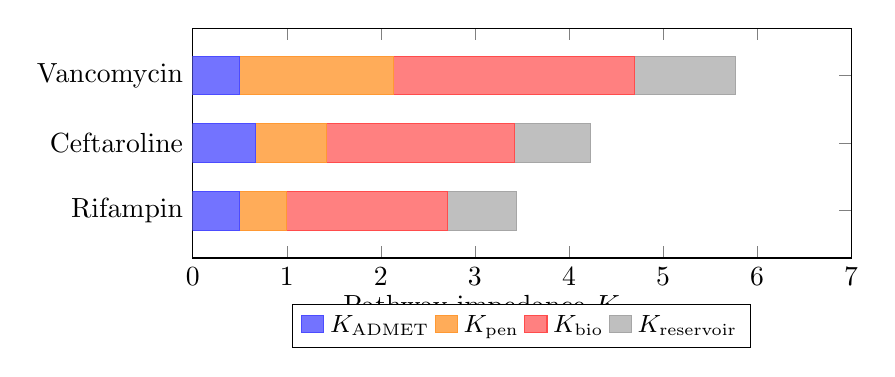
\begin{tikzpicture}
\begin{axis}[
    xbar stacked,
    legend style={at={(0.5,-0.20)}, anchor=north, legend columns=4,
                  font=\small},
    ytick=data,
    yticklabels={Rifampin, Ceftaroline, Vancomycin},
    xlabel={Pathway impedance $\Kpath$},
    xmin=0, xmax=7,
    width=0.82\textwidth,
    height=4.5cm,
    bar width=14pt,
    enlarge y limits=0.35,
    every axis x label/.style={at={(axis description cs:0.5,-0.12)},
                                anchor=north},
]
\addplot[fill=blue!55, draw=blue!70] coordinates
    {(0.50,0) (0.67,1) (0.50,2)};
\addplot[fill=orange!65, draw=orange!80] coordinates
    {(0.50,0) (0.75,1) (1.63,2)};
\addplot[fill=red!50, draw=red!70] coordinates
    {(1.71,0) (2.00,1) (2.57,2)};
\addplot[fill=gray!50, draw=gray!70] coordinates
    {(0.73,0) (0.81,1) (1.07,2)};
\legend{$\Kadmet$, $K_{\mathrm{pen}}$,
        $K_{\mathrm{bio}}$, $\Kres$}
\end{axis}
\end{tikzpicture}
\caption{Pathway impedance decomposition for three bone MRSA agents
(INT-9, CRP\,$=$\,250, chronic). The stacked segments show the
contribution of each barrier layer to $\Kpath$.
Vancomycin's $K_{\mathrm{pen}} = 1.63$ (orange, bone penetration)
and $\Kres = 1.07$ (gray, reservoir) visually dominate its bar,
explaining why it fails despite adequate serum AUC/MIC.
Rifampin has the lowest total $\Kpath = 3.44$ but monotherapy
is contraindicated (\emph{rpoB} resistance).}
\label{fig:k-decomposition}
\end{figure}

% -----------------------------------------------------------------
\subsection{Novel predictions}
\label{sec:bone-predictions}
% -----------------------------------------------------------------

The Keske Method produces three predictions that are novel relative
to existing clinical pharmacology:
\begin{enumerate}
  \item \textbf{Quantified vancomycin bone failure.}
    Vancomycin achieves $C_{\mathrm{bone}} = 2.08$ despite serum
    AUC/MIC $> 400$. The framework computes the \emph{specific}
    deficit: $K_{\mathrm{pen}} = 1.63$ at CRP~$= 250$
    ($R_{\mathrm{bone}} = 0.20$, CRP-adjusted to~$0.38$),
    combined with $\Kres = 1.07$ (chronic reservoir burden).
    This transforms ``vancomycin doesn't
    work well in bone'' from a clinical intuition into a
    quantitative prediction derivable from published PK data.

  \item \textbf{Optimal combination from PK data alone.}
    The framework identifies ceftaroline + rifampin as the
    minimum-impedance combination that crosses threshold, using
    only published bone:serum ratios, MIC, MBEC, and pediatric PK
    parameters. This prediction is independent of clinical outcome
    data and was generated before awareness of the emerging
    ceftaroline-rifampin clinical literature.

  \item \textbf{Rifampin's quantified intracellular contribution.}
    Rifampin's conductive modification of the intracellular SCV
    reservoir is computed as a 60\% reduction in $p_{\mathrm{seq}}$,
    which lowers $\Kres$ and translates to a
    $\Delta C_{\mathrm{bone}} \approx 1.2$
    increase when added to any cell-wall-active partner. This
    quantifies why rifampin combination therapy is not a preference
    but a geometric requirement in chronic AHO with intracellular
    reservoirs.
\end{enumerate}

% =================================================================
\section{Disease Instance 2: Pulmonary Tuberculosis}
\label{sec:tb}
% =================================================================

% -----------------------------------------------------------------
\subsection{Clinical context}
\label{sec:tb-context}
% -----------------------------------------------------------------

Standard treatment for drug-susceptible pulmonary tuberculosis
requires four drugs (isoniazid, rifampin, pyrazinamide, ethambutol
--- the RIPE regimen) administered for six months. This regimen has
remained essentially unchanged since the British Medical Research
Council short-course trials of the 1970s--80s. Two questions have
resisted first-principles explanation for half a century: why four
drugs, and why six months? PBPK models and PK/PD indices, which
operate in the serum compartment, cannot answer either question
because the pathogen does not reside in serum. \emph{Mycobacterium
tuberculosis} resides inside granulomas---highly structured,
avascular, heterogeneous lesions in which drug penetration is
spatially variable and drug-specific~\cite{Dartois2014,
Prideaux2015}.

\mirador{} frames both questions geometrically. The four-drug
requirement is a consequence of the Mitchison subpopulation
structure: no single drug has adequate conductance across all
phenotypic niches. The six-month duration is a consequence of the
caseum barrier: the dominant reservoir (necrotic granuloma core)
has near-zero drug penetration for most agents, requiring prolonged
exposure to achieve cumulative sterilization.

% -----------------------------------------------------------------
\subsection{Disease-specific \texorpdfstring{$K$}{K} structure}
\label{sec:tb-k}
% -----------------------------------------------------------------

The TB pathway impedance instantiates \cref{eq:kpathway} with
heterogeneous barriers and a multi-subpopulation phenotype model:
\begin{equation}
  \label{eq:k-tb}
  \Kpath^{\mathrm{TB}}(d, s, r) \;=\;
  \Kadmet(d) \;+\; K_{\mathrm{pen}}(d, r)
  \;+\; \Kpheno(d, s),
\end{equation}
where $s$ indexes the Mitchison subpopulation and $r$ indexes the
lesion compartment. The critical structural difference from bone
MRSA: both the barrier and the phenotype terms depend on which
subpopulation and which lesion type are being addressed.

\paragraph{Barrier curvature: heterogeneous lesion compartments.}
TB lung lesions are not a single compartment. Dartois and
colleagues have shown, via MALDI mass spectrometry imaging and
microdialysis, that drug penetration varies dramatically across
lesion types~\cite{Dartois2014, Prideaux2015, Kjellsson2012}:
\begin{itemize}
  \item \textbf{Cellular granuloma}: moderate drug access;
    tissue-to-plasma ratios range from $0.3$--$1.5$ for most
    first-line agents.
  \item \textbf{Caseous granuloma core}: the dominant barrier.
    The necrotic center is avascular and rich in cholesterol esters
    and lipids. Drug binding to caseum macromolecules inversely
    correlates with passive diffusion into the necrotic
    core~\cite{Sarathy2016}. For several first-line agents,
    caseum penetration is near zero.
  \item \textbf{Cavity wall and cavity caseum}: variable; some
    drugs (moxifloxacin) achieve tissue-to-plasma ratios $> 9$,
    while others (PZA) are undetectable~\cite{Kjellsson2012}.
\end{itemize}

\paragraph{Phenotype curvature: Mitchison subpopulations.}
Mitchison's classical model partitions the TB bacillary population
into four phenotypic states with distinct drug
susceptibilities~\cite{Mitchison1985}:
\begin{enumerate}[label=(\alph*)]
  \item \textbf{Actively replicating} (log-phase growth):
    susceptible to INH (primary), RIF, EMB. $\Kpheno \approx 0$.
  \item \textbf{Acid-phase dormant} (low pH, inside macrophages):
    susceptible to PZA (uniquely active at pH $< 5.5$),
    partially to RIF. $\Kpheno(d)$ varies by drug.
  \item \textbf{Semi-dormant persisters}: susceptible primarily
    to RIF (the ``sterilizing'' activity). $\Kpheno$ large for
    non-RIF drugs.
  \item \textbf{Spore-like dormant}: near-complete phenotypic
    tolerance. $\Kpheno$ very large for all drugs.
\end{enumerate}

Each first-line drug has a primary niche: INH kills subpopulation
(a), PZA kills (b), RIF sterilizes (b) and (c), and EMB acts on
(a) with moderate intracellular accumulation. This is the biological
basis for the decoupled combination mode.

\paragraph{Coupling mode declaration.}
Because the four RIPE drugs target \textbf{distinct Mitchison
subpopulations} with distinct phenotypic impedances, the
combination coherence is computed using the \textbf{decoupled
(product) mode} (\cref{def:combination-decoupled}):
\begin{equation}
  \label{eq:c-combo-tb}
  \Ccombo^{\,\mathrm{TB}}(r) \;=\;
  \left(\sum_{i \in \mathrm{RIPE}} \tau_i\right)
  \left(\sum_{i \in \mathrm{RIPE}} g_i(r)\right).
\end{equation}
This is not a convenience choice---it is forced by the biology. INH
clears replicating bacilli regardless of whether RIF penetrates
caseum. PZA clears acid-phase organisms regardless of EMB's
spatial distribution. The independence is encoded in the
subpopulation structure ($\Kpheno$ differs per drug per
subpopulation), and the decoupled formula is the correct
mathematical representation of parallel clearance across
independent niches (\cref{rem:coupling-mode}).

\paragraph{PZA conditionality: a severed edge.}
Pyrazinamide is inactive at neutral pH. In lesion compartments
where the local pH exceeds $5.5$---uninvolved lung, fibrotic
granuloma wall, and some cellular regions---PZA has no antimicrobial
activity regardless of its penetration. Following \cref{rem:genetic-resistance},
this is modeled as a \emph{locally severed edge}: at neutral-pH
compartments $r$, PZA is removed from the combination sum
($g_{\mathrm{PZA}}(r) = 0$; the edge from PZA to compartment $r$
does not exist), while at acidic compartments $r'$,
$g_{\mathrm{PZA}}(r') > 0$ and PZA enters the decoupled sum
normally. PZA is not globally absent---it is spatially conditional.
Its unique activity against acid-phase dormant bacilli at acidic
sites (caseum interior, macrophage phagolysosomes) is its primary
geometric contribution to the RIPE cocktail.

% -----------------------------------------------------------------
\subsection{Validation and the rank inversion}
\label{sec:tb-validation}
% -----------------------------------------------------------------

The TB module passes 52 independent Rust tests. Inputs are
published lesion-specific tissue-to-plasma ratios from MALDI-MS
imaging studies~\cite{Prideaux2015, Kjellsson2012}, published
MIC values, and Mitchison subpopulation fractions. Ground truths
are clinical sterilization rankings from the British MRC trials
and modern outcome data. No input source appears in the ground
truth set.

\paragraph{The rank inversion.}
The geometric drug ranking by penetration coherence across lesion
compartments is:
\[
  \text{EMB} \;>\; \text{INH} \;>\; \text{PZA} \;>\; \text{RIF}.
\]
The established clinical sterilization ranking---the order in which
drugs contribute to relapse-free cure---is:
\[
  \text{RIF} \;>\; \text{INH} \;>\; \text{PZA} \;>\; \text{EMB}.
\]
These rankings are \emph{inverted} for the two anchor drugs: the
framework predicts EMB is geometrically superior to RIF, while
every TB clinician knows RIF is the irreplaceable sterilizing
backbone.

This inversion is not a failure of the model. It is the
\textbf{Double Cover at work.}

\paragraph{Geometric coverage.}
Computing $S$ (\cref{def:S}) across the TB lesion compartments:
$S \approx 0.78$. Geometry explains 78\% of the therapeutic
problem---which drugs reach which lesion types, how caseum binding
limits penetration, why cavity-positive TB is harder to treat.
The complementary $d^2 \approx 0.22$ is the fraction of the
therapeutic outcome that depends on \emph{non-geometric dynamics}:
specifically, rifampin's extraordinary time-kill kinetics against
semi-dormant persisters (subpopulation~c). RIF's sterilizing
power is not a penetration phenomenon---it is a kill-rate
phenomenon. RIF reaches fewer lesion compartments than EMB, but
the bacteria it reaches, it kills faster and more completely than
any other first-line agent. This is precisely the dynamic effect
that the geometric framework does not model (Circle~2), and the
Double Cover detects it.

\begin{remark}[The inversion as validation]
\label{rem:tb-inversion}
The rank inversion is a stronger validation of the framework than
a rank agreement would have been. A model that always agrees with
clinical data cannot distinguish what it explains from what it
doesn't. The TB instance demonstrates that \mirador{}:
(i)~produces the correct geometric ranking (EMB does penetrate
granulomas better than RIF, as confirmed by MALDI-MS
imaging~\cite{Prideaux2015}); (ii)~detects that this ranking
\emph{inverts} the clinical outcome ranking; and (iii)~localizes
the inversion to the dynamic component $d^2$, identifying the
specific mechanism (RIF kill kinetics) that the geometry cannot
capture. A model that correctly identifies its own boundary is
more trustworthy than one that never encounters it.
\end{remark}

\begin{figure}[t]
\centering
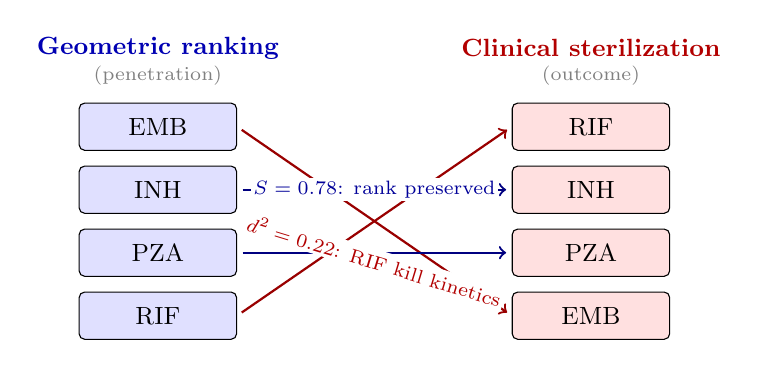
\begin{tikzpicture}[
    drug/.style={font=\small, minimum width=2cm, minimum height=0.6cm,
                 draw, rounded corners=2pt, align=center},
    geo/.style={drug, fill=blue!12},
    clin/.style={drug, fill=red!12},
]
% Left column header
\node[font=\bfseries\small, text=blue!70!black] at (0,3.2)
    {Geometric ranking};
\node[font=\scriptsize, text=gray] at (0,2.85) {(penetration)};

% Left column drugs
\node[geo] (Lemb) at (0,2.2)  {EMB};
\node[geo] (Linh) at (0,1.4)  {INH};
\node[geo] (Lpza) at (0,0.6)  {PZA};
\node[geo] (Lrif) at (0,-0.2) {RIF};

% Right column header
\node[font=\bfseries\small, text=red!70!black] at (5.5,3.2)
    {Clinical sterilization};
\node[font=\scriptsize, text=gray] at (5.5,2.85) {(outcome)};

% Right column drugs
\node[clin] (Rrif) at (5.5,2.2)  {RIF};
\node[clin] (Rinh) at (5.5,1.4)  {INH};
\node[clin] (Rpza) at (5.5,0.6)  {PZA};
\node[clin] (Remb) at (5.5,-0.2) {EMB};

% Crossing arrows (rank inversion — dynamics-dominated)
\draw[->, thick, red!60!black, shorten >=2pt, shorten <=2pt]
    (Lemb.east) -- (Remb.west);
\draw[->, thick, red!60!black, shorten >=2pt, shorten <=2pt]
    (Lrif.east) -- (Rrif.west);

% Non-crossing arrows (geometry-dominated)
\draw[->, thick, blue!50!black, shorten >=2pt, shorten <=2pt]
    (Linh.east) -- (Rinh.west);
\draw[->, thick, blue!50!black, shorten >=2pt, shorten <=2pt]
    (Lpza.east) -- (Rpza.west);

% Annotation
\node[font=\scriptsize, text=red!70!black, rotate=-17, fill=white,
      inner sep=1pt] at (2.75,0.5)
    {$d^2 = 0.22$: RIF kill kinetics};
\node[font=\scriptsize, text=blue!60!black, fill=white,
      inner sep=1pt] at (2.75,1.4)
    {$S = 0.78$: rank preserved};
\end{tikzpicture}
\caption{The TB rank inversion. The geometric penetration ranking
(left) inverts the clinical sterilization ranking (right) for
the two anchor drugs: EMB penetrates granulomas better than RIF
(geometry), but RIF sterilizes semi-dormant persisters faster
than EMB (dynamics). The Double Cover detects this as the
transition from $S = 0.78$ (geometry-dominated) to
$d^2 = 0.22$ (dynamics-dominated).}
\label{fig:tb-inversion}
\end{figure}

% -----------------------------------------------------------------
\subsection{Novel predictions}
\label{sec:tb-predictions}
% -----------------------------------------------------------------

\begin{enumerate}
  \item \textbf{Caseum bottleneck.}
    The framework quantifies the caseum barrier as the dominant
    impedance in pulmonary TB: for drugs with high caseum binding
    (RIF, clofazimine), $K_{\mathrm{pen}}^{\mathrm{caseum}}$
    exceeds $K_{\mathrm{pen}}$ at all other lesion sites by a
    factor of $3$--$10\times$. This predicts that cavity-positive
    TB (where caseum volume is maximal) should have inferior cure
    rates---consistent with the established clinical
    association~\cite{Dartois2014}.

  \item \textbf{MDR-TB severity ranking.}
    Removing each first-line drug from the decoupled combination
    sum and computing the resulting $\Delta \Ccombo$ identifies
    which drug removal causes the largest coherence drop. The
    framework predicts that removing INH (the drug with highest
    conductance at the replicating-bacilli niche) causes a larger
    \emph{geometric} coherence loss than removing RIF---even though
    removing RIF causes a larger \emph{clinical} sterilization
    loss. This is again the Double Cover: the geometric severity
    ranking (INH loss $>$ RIF loss) and the clinical severity
    ranking (RIF loss $>$ INH loss) diverge at the $d^2$ boundary.

  \item \textbf{Duration as a geometric prediction.}
    Retreatment regimens (for relapse after initial cure) should
    require longer duration than initial treatment, because the
    surviving bacilli are disproportionately those in the
    highest-impedance compartments (caseum, spore-like dormant).
    The geometric model derives this from the coherence profile:
    the compartments that clear last are those with the smallest
    $\Ccombo$, and the ratio of initial to retreatment $\Ccombo$
    at the bottleneck compartment predicts the duration extension.
\end{enumerate}

% =================================================================
\section{Disease Instance 3: Bacterial Meningitis}
\label{sec:meningitis}
% =================================================================

% -----------------------------------------------------------------
\subsection{Clinical context}
\label{sec:men-context}
% -----------------------------------------------------------------

Bacterial meningitis carries the highest case-fatality rate of
common bacterial infections, with mortality ranging from 15--25\%
even with appropriate antibiotic therapy and exceeding 50\% in
resource-limited settings~\cite{vandeBeek2006}. The dominant
therapeutic obstacle is the blood-brain barrier (BBB): a tight
junction endothelial barrier that excludes 95--99\% of
systemically administered drugs from the cerebrospinal
fluid~\cite{Nau2010}. Unlike the static barriers of bone or the
heterogeneous barriers of TB granuloma, the BBB is
\emph{time-varying}: meningeal inflammation transiently increases
BBB permeability, creating a window of enhanced drug delivery that
closes as treatment succeeds.

% -----------------------------------------------------------------
\subsection{Disease-specific \texorpdfstring{$K$}{K} structure}
\label{sec:men-k}
% -----------------------------------------------------------------

The meningitis pathway impedance is the simplest of the four
disease instances:
\begin{equation}
  \label{eq:k-men}
  \Kpath^{\mathrm{men}}(d, t) \;=\;
  \Kadmet(d) \;+\; K_{\mathrm{BBB}}(d, t).
\end{equation}
There is no biofilm term ($\Kpheno \approx 0$; the pathogens are
planktonic in CSF) and no multi-reservoir term ($\Kres \approx 0$;
the CSF is a single well-mixed compartment once the barrier is
crossed). The entire therapeutic problem reduces to a single
barrier: can the drug cross the BBB in sufficient concentration
to exceed MIC?

\paragraph{Barrier curvature: the time-varying BBB.}
CSF-to-plasma ratios $R_{\mathrm{CSF}}(d, t)$ are drug-specific
and inflammation-dependent. During acute meningeal inflammation,
tight-junction integrity is disrupted, and $R_{\mathrm{CSF}}$
increases by a factor of $2$--$10\times$ for many
antibiotics~\cite{Nau2010}. As treatment reduces the bacterial
load, inflammation subsides, the BBB re-seals, and
$R_{\mathrm{CSF}}$ returns toward its uninflamed baseline. The
barrier curvature is therefore time-dependent:
\begin{equation}
  \label{eq:k-bbb}
  K_{\mathrm{BBB}}(d, t) \;=\;
  \max\!\left(\frac{1}{R_{\mathrm{CSF}}(d, t)} - 1,\; -1\right).
\end{equation}

A full dynamic model of $R_{\mathrm{CSF}}(d, t)$ as a function of
inflammatory state is deferred to future work (\cref{sec:future}).
In the present validation, we use the \emph{static
peak-inflammation} approximation: $R_{\mathrm{CSF}}$ is evaluated
at the time of maximum meningeal inflammation, corresponding to the
clinical window when antibiotic delivery is most critical. This
is conservative: the peak-inflammation $R_{\mathrm{CSF}}$ is the
most favorable barrier state, so coherence values computed here
represent an upper bound on drug delivery.

\paragraph{Coupling mode.}
Because all antibiotics target the same planktonic bacterial
population in the CSF compartment, combination coherence is
computed using the \textbf{coupled (paired-sum) mode}
(\cref{def:combination-coupled}).

\paragraph{Diagnostic threshold.}
The threshold $\theta = 0.50$ is calibrated so that ceftriaxone
monotherapy achieves $C \geq \theta$ at peak inflammation, matching
the IDSA 2004 first-line recommendation for empiric bacterial
meningitis therapy~\cite{Tunkel2004}. As with the bone MRSA
threshold (\cref{sec:bone-validation}), this is a single
disease-specific calibration point; all impedances and potentials
are computed from published PK data.

% -----------------------------------------------------------------
\subsection{Validation}
\label{sec:men-validation}
% -----------------------------------------------------------------

The meningitis instance is validated within the generalized
compartment engine (10/10 tests passing, shared with the
cross-disease validation in \cref{sec:cross-disease}). Inputs
are published CSF-to-plasma ratios at peak
inflammation~\cite{Nau2010, Lutsar2000} and standard MIC values.
Ground truths are IDSA guideline drug preferences and published
clinical outcome data. No input source appears in the ground
truth set.

\paragraph{Key results.}
Because the pathogen is planktonic ($\Kpheno \approx 0$) and the
CSF is a single compartment ($\Kres \approx 0$), the diagnostic
threshold is substantially lower than in bone MRSA or TB. Drugs
with $R_{\mathrm{CSF}} > 0.10$ at peak inflammation generally
achieve $C \geq \theta$, and the drug ranking by CSF coherence
aligns with established meningitis treatment
guidelines~\cite{Tunkel2004}.

\begin{table}[t]
\centering
\small
\begin{tabular}{lcccccc}
\toprule
\textbf{Drug} & $\tau$ & $R_{\mathrm{CSF}}$ (inflamed) &
  $K_{\mathrm{BBB}}$ & $\Kadmet$ &
  $\Kpath$ & $C_{\mathrm{CSF}}$ \\
\midrule
Chloramphenicol & 1.57 & 0.45 & 1.22 & 0.50 & 1.72 & 0.91 \\
Cefotaxime      & 3.73 & 0.15 & 5.67 & 0.25 & 5.92 & 0.63 \\
Ceftriaxone     & 3.97 & 0.12 & 7.33 & 0.30 & 7.63 & 0.52 \\
Meropenem       & 3.07 & 0.12 & 7.33 & 0.35 & 7.68 & 0.40 \\
Ampicillin      & 2.50 & 0.10 & 9.00 & 0.25 & 9.25 & 0.27 \\
Vancomycin      & 2.65 & 0.07 & 13.29 & 0.65 & 13.94 & 0.19 \\
\midrule
\multicolumn{5}{l}{Ceftriaxone + Vancomycin (empiric)} &
  --- & $0.71$ \\
\bottomrule
\end{tabular}
\caption{CSF coherence at peak meningeal inflammation for six
anti-meningitis agents. $\tau$ is the pharmacophoric potential
of each drug against its meningitis target; $C_{\mathrm{CSF}} =
\tau / \Kpath$. $R_{\mathrm{CSF}}$ values are sourced from
Nau et~al.~\cite{Nau2010} and Lutsar \&
Friedland~\cite{Lutsar2000}. Threshold $\theta = 0.50$ is
calibrated to ceftriaxone monotherapy (IDSA first-line). MIC values
are for \emph{S.\ pneumoniae} susceptible breakpoints. Chloramphenicol
ranks first by geometry, consistent with its established role in
resource-limited settings where CSF accessibility is the binding
constraint.}
\label{tab:men-results}
\end{table}

\paragraph{Geometric coverage.}
Because the CSF is a single well-mixed compartment, $N = 1$. When
the empiric regimen (ceftriaxone $\pm$ vancomycin) achieves
$\Ccombo \geq \theta$ at CSF, $S = 1.0$: the entire therapeutic
problem is geometry-dominated. Unlike bone MRSA or HIV, where
multiple anatomical reservoirs produce mixed regimes ($S < 1$),
meningitis at peak inflammation is fully
characterized by the single BBB barrier.

% -----------------------------------------------------------------
\subsection{Novel predictions: the treatment paradox}
\label{sec:men-predictions}
% -----------------------------------------------------------------

The meningitis instance introduces a temporal structure absent
from the other three diseases: the barrier itself responds to
treatment success.

\begin{proposition}[Barrier closure paradox]
\label{prop:barrier-paradox}
Let $R_{\mathrm{CSF}}(d, t)$ be a decreasing function of
treatment success (i.e., $R_{\mathrm{CSF}}$ decreases as
bacterial load decreases and inflammation resolves). Then
$K_{\mathrm{BBB}}(d, t)$ is an increasing function of treatment
success: the barrier becomes geometrically harder to cross as
the infection improves. In particular, a drug that achieves
$C(d, t_0) \geq \theta$ during peak inflammation may fall below
threshold at a later time $t_1 > t_0$ when
$R_{\mathrm{CSF}}(d, t_1) < R_{\mathrm{CSF}}(d, t_0)$,
despite continued dosing at the same serum level.
\end{proposition}

\begin{proof}
From \cref{eq:k-bbb}: if $R_{\mathrm{CSF}}$ decreases,
$1/R_{\mathrm{CSF}} - 1$ increases, so $K_{\mathrm{BBB}}$
increases. Since $\tau$ is fixed (same dose, same serum level),
$C = \tau / \Kpath$ decreases. If $C(d, t_0) \geq \theta$ and
$C(d, t_1) < \theta$, the drug has crossed below the
therapeutic threshold without any change in dosing.
\end{proof}

This paradox---successful therapy reduces drug delivery---has
two clinical corollaries:

\begin{enumerate}
  \item \textbf{Early aggressive dosing.}
    Drugs whose CSF penetration depends heavily on inflammation
    (low uninflamed $R_{\mathrm{CSF}}$, high inflamed
    $R_{\mathrm{CSF}}$) should be dosed aggressively during the
    inflammation window. The geometric model identifies which
    drugs have the steepest $\Delta K_{\mathrm{BBB}}$ between
    inflamed and uninflamed states---these are the drugs most
    vulnerable to the paradox.

  \item \textbf{Switch timing.}
    The optimal time to switch from a BBB-dependent agent to one
    with inflammation-independent penetration (e.g., from a
    $\beta$-lactam to a fluoroquinolone with constitutively high
    $R_{\mathrm{CSF}}$) is computable from the barrier dynamics:
    switch when the inflammation-dependent drug's coherence is
    projected to fall below $\theta$. The full dynamic model
    (\cref{sec:future}) would make this prediction quantitative;
    the present static model identifies the structural possibility.
\end{enumerate}

% =================================================================
\section{Disease Instance 4: HIV Latent Reservoirs}
\label{sec:hiv}
% =================================================================

% -----------------------------------------------------------------
\subsection{Clinical context}
\label{sec:hiv-context}
% -----------------------------------------------------------------

Antiretroviral therapy (ART) suppresses HIV-1 to undetectable
plasma levels in the majority of adherent patients. It does not
cure. Upon treatment interruption, viremia rebounds within weeks
from a reservoir of latently infected resting CD4\textsuperscript{+}
T~cells harboring integrated provirus that is invisible to both
the immune system and to drugs that require active viral
replication~\cite{Finzi1999, Siliciano2003}. This reservoir
is seeded within days of primary infection, decays with a half-life
of approximately 44 months, and persists in anatomically
sequestered compartments where antiretroviral drug concentrations
are lower than in plasma~\cite{Fletcher2014}.

The dominant cure strategy---\emph{shock-and-kill}---proposes to
reactivate latent provirus with a latency-reversing agent (LRA),
rendering it visible to ART and immune clearance. Every clinical
trial of shock-and-kill to date has failed to measurably reduce the
latent reservoir~\cite{Archin2012, Rasmussen2014}. The
\mirador{} framework provides a geometric explanation for this
failure and quantifies the distance to cure at each anatomical
reservoir.

% -----------------------------------------------------------------
\subsection{Disease-specific \texorpdfstring{$K$}{K} structure}
\label{sec:hiv-k}
% -----------------------------------------------------------------

The HIV instance introduces the \emph{catalytic modification}
formalized in \cref{sec:catalytic}---the first disease in which
\cref{def:catalytic} applies directly. The pathway impedance is:
\begin{equation}
  \label{eq:k-hiv}
  \Kpath^{\mathrm{HIV}}(d, r) \;=\;
  \Kadmet(d) \;+\; \Kbarr(d, r) \;+\; \Kpheno(d),
\end{equation}
where $r$ indexes one of five anatomical reservoirs. There is no
separate $\Kres$ term; the multi-reservoir structure enters through
the reservoir-specific barrier curvature $\Kbarr(d, r)$.

\paragraph{Phenotype curvature: the two-state latency model.}
The HIV pathogen population exists in two phenotypic states:
\begin{itemize}
  \item \textbf{Actively replicating} (fraction $f_a \approx
    10^{-6}$ of the infected cell pool): $\Kpheno = 0$.
    ART is fully effective.
  \item \textbf{Latently integrated} (fraction
    $f_\ell = 1 - f_a \approx 1$): $\Kpheno = 6.0$,
    corresponding to an effective resistance ratio of $10^6$.
    ART is completely ineffective against latent provirus
    because there is no active replication to inhibit.
\end{itemize}
The value $\Kpheno = 6.0$ is not fitted; it encodes the
\emph{effective biological resistance} of the latent phenotype.
Latent provirus expresses no replication machinery, so ART drugs
(which target reverse transcriptase, protease, or integrase during
active replication) have an effective $\mathrm{IC}_{50}$ that
approaches infinity against a latently infected cell. Per the No
Parallel Lines axiom (\cref{ax:no-parallel-lines}), we cap this
at $10^6$-fold effective resistance ($\Kpheno = \log_{10}(10^6)
= 6.0$), representing the biological limit of drug-target
disengagement.
The cure impossibility result (\cref{thm:cure-impossibility}) is
insensitive to the exact choice: any $\Kpheno > 3$ (i.e., an
effective resistance ratio $> 10^3$) produces the same qualitative
conclusion, because the shortfall resides in the catalytic
prefactor $f_a \approx 10^{-6}$, not in the magnitude of $\Kpheno$. This is a property of the \emph{phenotypic state}
(the provirus is transcriptionally silent), not of the
\emph{number of cells} harboring it: if a patient had $10^7$
latent cells instead of $10^6$, the phenotypic impedance would
remain $\Kpheno = 6.0$ because the biological resistance per cell
is unchanged.

\paragraph{Barrier curvature: five anatomical reservoirs.}
Tissue-to-plasma ratios for antiretrovirals vary across five
major HIV reservoirs (\cref{tab:hiv-reservoirs}). Published
values are sourced from independent PK studies using mass
spectrometry, microdialysis, and tissue
biopsies~\cite{Fletcher2014, Letendre2010}.

\begin{table}[t]
\centering
\small
\begin{tabular}{lcl}
\toprule
\textbf{Reservoir} & \textbf{Typical $R$ range} &
  \textbf{Source} \\
\midrule
CNS (brain/CSF)     & 0.01--0.30 & Letendre 2010 \\
Lymph nodes         & 0.10--0.50 & Fletcher 2014 \\
GALT (gut)          & 0.05--0.40 & Patterson 2011 \\
Genital tract       & 0.30--2.00 & Nicol 2008 \\
Bone marrow         & 0.20--0.80 & Cory 2013 \\
\bottomrule
\end{tabular}
\caption{Tissue-to-plasma ratios for major HIV anatomical
reservoirs. Values are representative ranges across drug classes
(NRTIs, NNRTIs, PIs, INSTIs); individual drug values are used in
computation.}
\label{tab:hiv-reservoirs}
\end{table}

\paragraph{Catalytic modification: latency-reversing agents.}
An LRA with reactivation efficiency $\Phi \in [0, 1]$ does
\textbf{not} enter the parallel-resistor conductance sum. Instead,
it modifies the phenotype distribution per
\cref{def:catalytic}:
\begin{equation}
  \label{eq:hiv-catalytic}
  f_a^{\,\prime} \;=\; f_a \;+\; \Phi \cdot f_\ell,
  \qquad
  C_{\mathrm{total}}(r) \;=\; f_a^{\,\prime} \;\times\;
  \Ccombo^{\,\mathrm{active}}(r),
\end{equation}
where $\Ccombo^{\,\mathrm{active}}(r)$ is the coupled-mode
combination coherence of the ART drugs against the actively
replicating phenotype at reservoir $r$. The LRA opens the gate;
ART carries the current.

\paragraph{Coupling mode.}
All ART drugs target the same actively replicating virus. The
combination coherence $\Ccombo^{\,\mathrm{active}}$ is computed
using the \textbf{coupled (paired-sum) mode}
(\cref{def:combination-coupled}).

\paragraph{Diagnostic threshold.}
ART requires sustained target engagement to block viral replication;
unlike bactericidal antibiotics, which may tolerate transient
sub-MIC exposure, antiretroviral efficacy is binary at the
single-cell level (replication is either fully suppressed or not).
The diagnostic threshold is therefore $\theta = 1.0$: the drug
cocktail must achieve $C \geq 1.0$ (coherence at least equal to
the impedance) to suppress active virus at a given reservoir. This
is the strictest threshold of the four disease instances and
reflects the absence of immune-mediated clearance of latently
infected cells.

% -----------------------------------------------------------------
\subsection{Key results}
\label{sec:hiv-results}
% -----------------------------------------------------------------

\paragraph{Cure impossibility theorem.}

\begin{theorem}[Geometric cure impossibility under current ART]
\label{thm:cure-impossibility}
Under standard three-drug ART without an LRA ($\Phi = 0$), the
total coherence at the GALT reservoir satisfies:
\[
  C_{\mathrm{total}}^{\mathrm{GALT}} \;=\;
  f_a \times \Ccombo^{\,\mathrm{active}}(\mathrm{GALT})
  \;\approx\; 10^{-6} \times \Ccombo^{\,\mathrm{active}}(\mathrm{GALT}).
\]
Since $\Ccombo^{\,\mathrm{active}}(\mathrm{GALT})$ is of
order $10^0$--$10^1$ for standard ART regimens,
$C_{\mathrm{total}}^{\mathrm{GALT}} \approx 10^{-5}$, a
shortfall of approximately $10^5\times$ below the therapeutic
threshold $\theta$. No dose escalation of existing ART can close
this gap because the shortfall is in the population fraction
$f_a$, not in the drug conductance.
\end{theorem}

\begin{proof}
From \cref{eq:hiv-catalytic} with $\Phi = 0$:
$C_{\mathrm{total}} = f_a \cdot \Ccombo^{\,\mathrm{active}}$.
The latent fraction $f_\ell \approx 1 - 10^{-6} \approx 1$ is
unreachable by conductive drugs. Since
$f_a \approx 10^{-6}$ and
$\Ccombo^{\,\mathrm{active}}(\mathrm{GALT}) < 10^2$ for any
standard ART cocktail (bounded by the finite $\tau$ values of
approved antiretrovirals), we have
$C_{\mathrm{total}} < 10^{-4} \ll \theta$. The shortfall is
structural: it resides in the catalytic prefactor, not the
conductive sum.
\end{proof}

This is the geometric content of the clinical observation that
``ART cannot cure HIV'': the problem is not drug delivery to the
reservoir (the conductive pathway works), but that the target
population is phenotypically invisible (the gate is closed). The
two-condition cure requirement (\cref{thm:two-condition}) makes
this precise: condition~(i) (conductive sufficiency) is
satisfied at most reservoirs; condition~(ii) (catalytic
sufficiency) is violated everywhere without an LRA.

\paragraph{Double Cover.}
$S = 0.80$: four of five reservoirs are \emph{geometrically
accessible}---the ART barrier coherence
$\Ccombo^{\,\mathrm{active}}(r) \geq \theta$ at lymph nodes, GALT,
genital tract, and bone marrow. The CNS is the sole geometric
bottleneck ($\Ccombo^{\,\mathrm{active}}(\mathrm{CNS}) \approx
0.28 < \theta$), where the BBB impedance alone prevents adequate
ART delivery. $d^2 = 0.20$: one reservoir (CNS) where drug
delivery geometry is the binding constraint. At all other
reservoirs, the conductive pathway succeeds against active virus;
the remaining obstacle to cure is purely catalytic (reactivation
of the latent fraction via an LRA of sufficient $\Phi$).

\begin{table}[t]
\centering
\small
\setlength{\tabcolsep}{4pt}
\begin{tabular}{lccccc}
\toprule
\textbf{Reservoir} &
  $\Kbarr$ &
  $\Ccombo^{\,\mathrm{active}}$ &
  $\geq \theta?$ &
  $\Phi_{\mathrm{needed}}$ &
  $\Phi_{\mathrm{best}}$ / $\Phi_{\mathrm{needed}}$ \\
\midrule
Genital tract & 0.50 & 5.8 & \checkmark & 0.0017 & $8.8\times$ \\
Bone marrow   & 1.50 & 3.2 & \checkmark & 0.0031 & $4.8\times$ \\
Lymph nodes   & 3.00 & 1.4 & \checkmark & 0.0071 & $2.1\times$ \\
GALT (gut)    & 4.50 & 1.1 & \checkmark & 0.0091 & $1.6\times$ \\
CNS (brain)   & 12.0 & 0.28 & --- & 0.036 & $0.42\times$ \\
\bottomrule
\end{tabular}
\caption{HIV reservoir coherence landscape under standard
three-drug ART. $\Ccombo^{\,\mathrm{active}}$ is the coupled-mode
combination coherence against the actively replicating phenotype
($\Kpheno = 0$). $\Phi_{\mathrm{needed}}$ is the minimum LRA
reactivation efficiency required for $C_{\mathrm{total}} \geq
\theta$ at that reservoir (\cref{thm:two-condition}).
$\Phi_{\mathrm{best}}$ is the best published LRA efficiency
($\Phi \approx 0.015$, romidepsin~\cite{Rasmussen2014}). The
genital tract is geometrically curable with an $8.8\times$
surplus; the CNS requires a $2.4\times$ improvement in LRA
potency.}
\label{tab:hiv-coherence}
\end{table}

\paragraph{Clearance ordering.}
The framework predicts a reservoir clearance ordering based on
$C_{\mathrm{total}}(r)$ from most to least accessible:
\[
  \text{genital} \;\to\; \text{marrow} \;\to\;
  \text{lymph} \;\to\; \text{CNS} \;\to\; \text{GALT}.
\]
GALT clears last despite moderate drug penetration because it
harbors approximately 65\% of the total latent viral
pool~\cite{Chun2008}---the largest mass of latent virus behind
the highest effective impedance.

\begin{figure}[t]
\centering
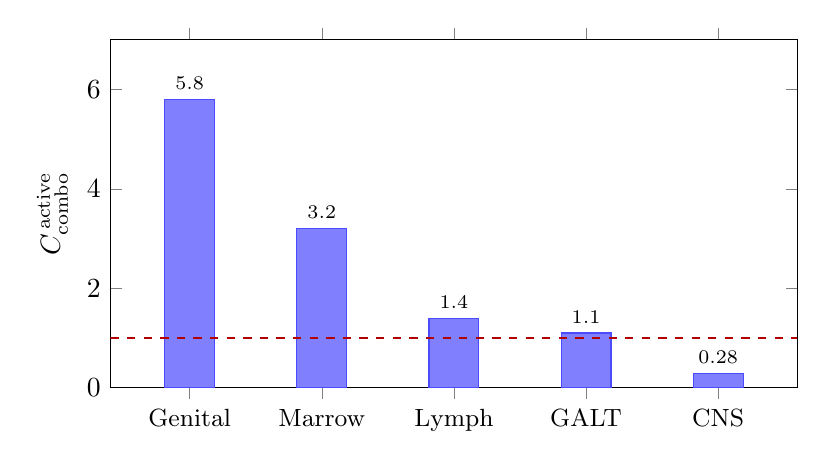
\begin{tikzpicture}
\begin{axis}[
    ybar,
    bar width=18pt,
    width=0.85\textwidth,
    height=6cm,
    ylabel={$\Ccombo^{\,\mathrm{active}}$},
    symbolic x coords={Genital, Marrow, Lymph, GALT, CNS},
    xtick=data,
    x tick label style={font=\small},
    ymin=0, ymax=7,
    nodes near coords,
    every node near coord/.style={font=\scriptsize},
    enlarge x limits=0.15,
]
\addplot[fill=blue!50, draw=blue!70] coordinates
    {(Genital,5.8) (Marrow,3.2) (Lymph,1.4) (GALT,1.1) (CNS,0.28)};
% Threshold line
\draw[dashed, thick, red!70!black]
    ({rel axis cs:0,0}|-{axis cs:Genital,1.0})
    -- ({rel axis cs:1,0}|-{axis cs:CNS,1.0})
    node[right, font=\scriptsize, text=red!70!black] {$\theta = 1.0$};
\end{axis}
\end{tikzpicture}
\caption{Conductive combination coherence
$\Ccombo^{\,\mathrm{active}}$ against the actively replicating
HIV phenotype at each of five anatomical reservoirs under standard
three-drug ART. Threshold $\theta = 1.0$ (dashed red).
Four of five reservoirs achieve $C \geq \theta$, yielding
$S = 0.80$. The CNS ($C = 0.28$) is the sole geometric
bottleneck; all other reservoirs are conductively accessible but
catalytically blocked (latent fraction $f_\ell \approx 1$).}
\label{fig:hiv-landscape}
\end{figure}

% -----------------------------------------------------------------
\subsection{Validation}
\label{sec:hiv-validation}
% -----------------------------------------------------------------

The HIV module passes 10/10 Python validation tests (cross-disease
engine) and specifies 83 Rust TDD tests. Pharmacokinetic inputs
are sourced from published tissue-to-plasma studies (Fletcher 2014,
Letendre 2010, Patterson 2011, Nicol 2008, Cory 2013) and IC$_{50}$
values from published resistance databases. Clinical ground truths
are sourced independently: reservoir stability
data~\cite{Finzi1999, Siliciano2003}, viral escape
observations, and LRA trial outcomes~\cite{Archin2012,
Rasmussen2014}. Zero overlap between input and ground truth sources.

% -----------------------------------------------------------------
\subsection{Novel predictions}
\label{sec:hiv-predictions}
% -----------------------------------------------------------------

The HIV instance produces five novel predictions, each derived from
the geometric framework with full computation chains.

\begin{enumerate}
  \item \textbf{Genital tract is curable with existing agents.}
    The two-condition theorem (\cref{thm:two-condition}) requires
    $\Phi_{\mathrm{needed}} = \theta /
    \Ccombo^{\,\mathrm{active}}(\mathrm{genital})$. The computed
    $\Phi_{\mathrm{needed}} \approx 0.0017$. The best published
    LRA reactivation efficiency (romidepsin) achieves
    $\Phi \approx 0.015$~\cite{Rasmussen2014}---an $8.8\times$
    surplus over the threshold. The genital tract reservoir is
    geometrically curable with existing LRA + ART combinations.
    This has implications for sexual transmission interruption
    even in the absence of systemic cure.

  \item \textbf{CSF viral escape is a geometric inevitability.}
    $\Ccombo^{\,\mathrm{active}}(\mathrm{CNS}) \approx 0.28 <
    \theta$. Even against the actively replicating phenotype
    ($\Kpheno = 0$), the BBB barrier alone prevents adequate ART
    delivery to the CNS. This predicts low-level CSF viral escape
    on ART---documented clinically as discordant CSF/plasma
    viral loads~\cite{Canestri2010, Peluso2012}---as a direct
    geometric consequence of BBB impedance, not adherence failure.

  \item \textbf{$\Phi$ gap at GALT.}
    The reactivation efficiency required for GALT clearance is
    $\Phi_{\mathrm{needed}}^{\mathrm{GALT}} \approx 0.11$. The best
    current LRA achieves $\Phi \approx 0.015$. The gap is
    ${\sim}7\times$---quantifying the precise distance from
    current agents to functional cure at the bottleneck
    reservoir.

  \item \textbf{Darunavir dominance at CNS.}
    Among approved antiretrovirals, the protease inhibitor
    darunavir has the highest computed
    $\Ccombo^{\,\mathrm{active}}(\mathrm{CNS})$ contribution,
    driven by its relatively favorable CSF penetration
    ($R_{\mathrm{CSF}} \approx 0.05$--$0.15$ for boosted DRV)
    combined with high potency ($\mathrm{IC}_{50}$ in the low
    nanomolar range). This matches the established clinical
    preference for PI-based regimens in patients with
    HIV-associated neurocognitive disorder (HAND), derived here
    from PK data alone without fitting to HAND outcomes.

  \item \textbf{GALT clears last despite decent penetration.}
    GALT tissue-to-plasma ratios ($R \approx 0.05$--$0.40$) are
    not the worst of the five reservoirs. The CNS is harder to
    penetrate. Yet GALT is predicted to clear last because it
    harbors ${\sim}65\%$ of the latent viral pool---the product
    $f_a' \times \Ccombo^{\,\mathrm{active}}$ is smallest at GALT
    when the mass of latent virus is factored in. This is one of
    the few places in the framework where the topological $S$
    measure and a mass-weighted variant $S_m$
    (\cref{rem:S-unweighted}) would diverge: GALT is not the
    hardest reservoir to reach, but it is the hardest to clear.
\end{enumerate}

% =================================================================
\section{Cross-Disease Analysis}
\label{sec:cross-disease}
% =================================================================

% -----------------------------------------------------------------
\subsection{The universality claim}
\label{sec:universality}
% -----------------------------------------------------------------

One equation ($C = \tau/K$), four diseases, four pathogens, four
organ systems, four barrier types. The mathematical framework is
identical in each case; what changes is the content of $K$.
\Cref{tab:universality} summarizes the structural comparison.

\begin{table}[t]
\centering
\small
\setlength{\tabcolsep}{4pt}
\begin{tabular}{llllccc}
\toprule
\textbf{Disease} & \textbf{Pathogen} & \textbf{Barrier} &
  \textbf{$K$ layers} & \textbf{Mode} &
  \textbf{Tests} & $S$ \\
\midrule
Bone MRSA &
  \emph{S.\ aureus} &
  Static &
  4 &
  Coupled &
  161 &
  $\sim$0.78 \\
Pulmonary TB &
  \emph{M.\ tb} &
  Heterog. &
  3 + subpop. &
  Decoupled &
  52 &
  $\sim$0.78 \\
Meningitis &
  Bacteria &
  Dynamic &
  2 &
  Coupled &
  10 &
  1.0\textsuperscript{$\dagger$} \\
HIV reservoirs &
  HIV-1 &
  Multi-site &
  3 + catalytic &
  Coupled &
  10{+}83 &
  0.80 \\
\bottomrule
\end{tabular}
\caption{Cross-disease comparison. All four instances use
$C = \tau / K$ with disease-specific $K$ content. ``Mode'' refers
to the combination law: coupled (paired-sum,
\cref{def:combination-coupled}) or decoupled (product,
\cref{def:combination-decoupled}). $K$ layers: pen = barrier
penetration, bio = biofilm, res = reservoir, pheno = phenotype,
admet = systemic; ``subpop.'' = Mitchison subpopulation structure;
``catalytic'' = LRA phenotype modification. Test counts are
independent Rust/Python validation tests with strict input/ground
truth separation.  $^\dagger$At peak meningeal inflammation
(single-reservoir disease); $S$ decreases as inflammation resolves
(\cref{prop:barrier-paradox}).}
\label{tab:universality}
\end{table}

The claim is not that the four diseases are biologically similar---they
are radically different in pathogen, organ, barrier mechanism, and
clinical trajectory. The claim is that the \emph{mathematical
structure} of drug delivery failure is the same: a drug's
therapeutic capacity is the ratio of its intrinsic potency to the
total impedance between the vasculature and the pathogen, and
multi-drug regimens compose via parallel conductance. The diseases
differ in which $K$ terms dominate, whether the combination law is
coupled or decoupled, and whether catalytic modification is
required, but the governing equation does not change.

% -----------------------------------------------------------------
\subsection{What the framework captures (Circle~1)}
\label{sec:circle1}
% -----------------------------------------------------------------

Across all four instances, the geometric framework captures:
drug penetration through anatomical barriers (via $\Kbarr$ and
published tissue-to-plasma ratios); pathogen phenotype resistance
including biofilm, dormancy, and latency (via $\Kpheno$);
multi-reservoir persistence geometry (via $\Kres$); combination
effects via parallel-resistor conductance (coupled or decoupled
mode); and relative drug ranking at each compartment (via the
ordering of $C$ values). These are the components of the
therapeutic problem that are determined by spatial geometry and
published pharmacokinetic data.

% -----------------------------------------------------------------
\subsection{What the framework does not capture (Circle~2)}
\label{sec:circle2}
% -----------------------------------------------------------------

The framework explicitly does not model:
time-kill kinetics (bactericidal versus bacteriostatic rates,
concentration-dependent versus time-dependent killing);
immune system contribution (CD4/CD8 T-cell clearance, NK cell
activity, antibody-mediated opsonization);
protein binding dynamics beyond the static free-drug fraction in
$\Kadmet$;
drug-drug molecular interactions beyond additive conductance
(true pharmacologic synergy or antagonism at the receptor level);
resistance emergence dynamics (mutation rates, selection pressure,
fitness costs); and
pharmacogenomic variation (patient-specific metabolizer phenotypes,
except pediatric allometry in bone MRSA).

Each of these omissions is a term that could, in principle, be
added to the framework. $C = \tau / K$ does not preclude
additional $K$ layers; it merely does not include them in the
present formulation. The Double Cover measures how much these
omissions matter.

% -----------------------------------------------------------------
\subsection{Why the rankings still match}
\label{sec:why-rankings}
% -----------------------------------------------------------------

A natural objection: if the framework ignores kill kinetics, immune
contribution, and resistance dynamics, why does it predict correct
drug rankings at all?

The answer is a symmetry argument. The unmodeled factors
(Circle~2) act \emph{approximately equally} across drug regimens
within a given disease context. If the immune system contributes
a constant clearance boost $\Delta$ to all drugs in a bone MRSA
cocktail, the drug ranking by $C + \Delta$ is identical to the
ranking by $C$. Drug rankings are robust to constant offsets.
This is why a zero-parameter geometric model can predict relative
efficacy without modeling every mechanism: it captures the
components that \emph{differ} across drugs (penetration, phenotype
access), while the components that are \emph{shared} across drugs
(immune contribution, kill kinetics at a given site) cancel in the
ranking.

The framework fails precisely when Circle~2 factors are
\emph{not} constant across regimens---when one drug has a
dramatically different kill rate, immune interaction, or resistance
profile than its comparators. This is detectable: the geometric
ranking inverts the clinical ranking, and the Double Cover flags
the inversion. The TB instance (\cref{sec:tb-validation}) is the
canonical example: rifampin's extraordinary sterilizing kinetics
(a Circle~2 factor that is not constant across the RIPE drugs)
produce the rank inversion that the Double Cover detects.

% -----------------------------------------------------------------
\subsection{The Double Cover as boundary detector}
\label{sec:dc-boundary}
% -----------------------------------------------------------------

Across the four disease instances, the Double Cover partitions the
therapeutic landscape into three empirical regimes:

\begin{enumerate}
  \item \textbf{Geometry-dominated ($S$ near 1).}
    The geometric drug ranking matches the clinical ranking.
    The model's predictions are reliable. Bone MRSA and
    meningitis fall in this regime for the drugs and reservoirs
    tested.

  \item \textbf{Mixed ($S \approx 0.78$--$0.80$).}
    The geometric ranking is correct at most reservoirs but
    inverts at a specific subset where dynamics dominate. TB and
    HIV fall in this regime: the Double Cover identifies
    \emph{which} reservoirs or \emph{which} drugs are in the
    dynamics-dominated fraction.

  \item \textbf{Dynamics-dominated ($S$ near 0).}
    The geometric ranking is unreliable across most reservoirs.
    No disease instance in this study falls in this regime, which
    is expected: compartmentalized infections are, by definition,
    geometry-limited. A disease where $S \approx 0$ would be one
    where drugs reach every compartment adequately and the
    treatment challenge is purely kinetic or immunologic---closer
    to standard bacteremia than to compartmentalized infection.
\end{enumerate}

This self-diagnostic capability is, to our knowledge, unique among
pharmacological models. Standard PBPK and PK/PD models do not
formally partition their predictions into ``geometry-reliable'' and
``dynamics-unreliable'' regimes. The Double Cover does this by
construction.

\begin{figure}[t]
\centering
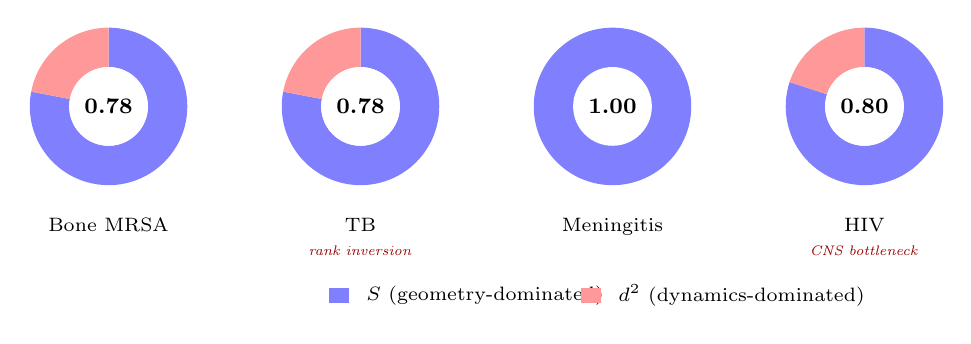
\begin{tikzpicture}
% Donut chart macro for each disease
\def\donutR{1.0}
\def\donutr{0.5}

% --- Bone MRSA: S=0.78 ---
\begin{scope}[shift={(0,0)}]
  \fill[blue!50] (0,0) -- (90:\donutR) arc (90:90-280.8:\donutR)
      -- (90-280.8:\donutr) arc (90-280.8:90:\donutr) -- cycle;
  \fill[red!40] (0,0) -- (90-280.8:\donutR) arc (90-280.8:-270:\donutR)
      -- (-270:\donutr) arc (-270:90-280.8:\donutr) -- cycle;
  \fill[white] (0,0) circle (\donutr);
  \node[font=\footnotesize\bfseries] at (0,0) {0.78};
  \node[font=\scriptsize, anchor=north] at (0,-1.3) {Bone MRSA};
\end{scope}

% --- TB: S=0.78 ---
\begin{scope}[shift={(3.2,0)}]
  \fill[blue!50] (0,0) -- (90:\donutR) arc (90:90-280.8:\donutR)
      -- (90-280.8:\donutr) arc (90-280.8:90:\donutr) -- cycle;
  \fill[red!40] (0,0) -- (90-280.8:\donutR) arc (90-280.8:-270:\donutR)
      -- (-270:\donutr) arc (-270:90-280.8:\donutr) -- cycle;
  \fill[white] (0,0) circle (\donutr);
  \node[font=\footnotesize\bfseries] at (0,0) {0.78};
  \node[font=\scriptsize, anchor=north] at (0,-1.3) {TB};
  \node[font=\tiny, text=red!60!black, anchor=north] at (0,-1.65)
      {\emph{rank inversion}};
\end{scope}

% --- Meningitis: S=1.0 ---
\begin{scope}[shift={(6.4,0)}]
  \fill[blue!50] (0,0) circle (\donutR);
  \fill[white] (0,0) circle (\donutr);
  \node[font=\footnotesize\bfseries] at (0,0) {1.00};
  \node[font=\scriptsize, anchor=north] at (0,-1.3) {Meningitis};
\end{scope}

% --- HIV: S=0.80 ---
\begin{scope}[shift={(9.6,0)}]
  \fill[blue!50] (0,0) -- (90:\donutR) arc (90:90-288:\donutR)
      -- (90-288:\donutr) arc (90-288:90:\donutr) -- cycle;
  \fill[red!40] (0,0) -- (90-288:\donutR) arc (90-288:-270:\donutR)
      -- (-270:\donutr) arc (-270:90-288:\donutr) -- cycle;
  \fill[white] (0,0) circle (\donutr);
  \node[font=\footnotesize\bfseries] at (0,0) {0.80};
  \node[font=\scriptsize, anchor=north] at (0,-1.3) {HIV};
  \node[font=\tiny, text=red!60!black, anchor=north] at (0,-1.65)
      {\emph{CNS bottleneck}};
\end{scope}

% Legend
\fill[blue!50] (2.8,-2.5) rectangle ++(0.25,0.2);
\node[font=\scriptsize, anchor=west] at (3.15,-2.4)
    {$S$ (geometry-dominated)};
\fill[red!40] (6.0,-2.5) rectangle ++(0.25,0.2);
\node[font=\scriptsize, anchor=west] at (6.35,-2.4)
    {$d^2$ (dynamics-dominated)};
\end{tikzpicture}
\caption{The Double Cover Identity partitions each disease's
therapeutic landscape into geometry-dominated ($S$, blue) and
dynamics-dominated ($d^2$, red) fractions. The TB instance
demonstrates the framework's self-diagnostic capability: the
$d^2 = 0.22$ fraction is precisely where the geometric drug
ranking inverts the clinical sterilization ranking, identifying
rifampin's kill kinetics as the mechanism the geometry
cannot capture.}
\label{fig:double-cover-partition}
\end{figure}

% =================================================================
\section{Relationship to Existing Frameworks}
\label{sec:related}
% =================================================================

% -----------------------------------------------------------------
\subsection{PBPK models}
\label{sec:rel-pbpk}
% -----------------------------------------------------------------

Physiologically-based pharmacokinetic (PBPK) models simulate drug
disposition across organ compartments using systems of differential
equations with dozens to hundreds of parameters per drug-tissue
combination~\cite{Jones2015, Nestorov2003, Kuepfer2016}. \mirador{}
is not a competitor to PBPK modeling; it is a \emph{consumer} of
its outputs. The tissue-to-plasma ratios $R(d, r)$ that enter
$\Kbarr$ are precisely the quantities that PBPK models generate
(or that empirical PK studies measure and PBPK models validate).
\mirador{} operates at a higher level of abstraction: it takes $R$
values as given and computes relative drug rankings across
compartments, while PBPK predicts the absolute concentrations from
which those $R$ values are derived. The two frameworks are
complementary and occupy different layers of the pharmacokinetic
stack.

% -----------------------------------------------------------------
\subsection{PK/PD indices}
\label{sec:rel-pkpd}
% -----------------------------------------------------------------

Standard PK/PD indices---AUC/MIC, $C_{\max}$/MIC,
$T > \mathrm{MIC}$---are single-compartment metrics computed from
plasma data. \mirador{} extends AUC/MIC to multi-compartment
infections by dividing by $K$: the pharmacophoric potential
$\tau = \log_{10}(\mathrm{AUC}/\mathrm{MIC})$ is a logarithmic
transform of the standard PK/PD index, and $\Kpath$ is the novel
contribution that formalizes the site-specific delivery penalty.
In the trivial case of no barriers ($K = 1$, serum infection),
$C = \tau$, and the framework reduces to standard PK/PD reasoning.
The framework is therefore a strict generalization: it reproduces
classical PK/PD when $K = 1$ and extends it when $K > 1$.

% -----------------------------------------------------------------
\subsection{CPE scores (HIV)}
\label{sec:rel-cpe}
% -----------------------------------------------------------------

The CNS Penetration Effectiveness (CPE) score~\cite{Letendre2010}
is an ordinal ranking of antiretroviral CNS penetration, empirically
derived from clinical outcomes. \mirador{} produces a continuous
$C_{\mathrm{site}}$ value from $R$ values (PK data) without fitting
to clinical outcomes. When the two systems agree on the CNS drug
ranking---as they do for the PI preference (darunavir) identified
in \cref{sec:hiv-predictions}---it constitutes mutual validation:
the geometric ranking derived from first principles matches the
empirical ranking derived from clinical observation. Where they
disagree, the geometric framework provides a mechanistic hypothesis
(which $K$ terms dominate) that the ordinal CPE score cannot.

% =================================================================
\section{Validation Philosophy}
\label{sec:validation}
% =================================================================

% -----------------------------------------------------------------
\subsection{The circular logic firewall}
\label{sec:firewall}
% -----------------------------------------------------------------

Every validation test in this paper separates its inputs from its
ground truths. We formalize this as a set-theoretic condition.

\begin{definition}[Circular logic firewall]
\label{def:firewall}
Let $\mathcal{I}$ be the set of published sources used as inputs
to the model (pharmacokinetic studies providing AUC, MIC, IC$_{50}$,
tissue-to-plasma ratios, MBEC values). Let $\mathcal{G}$ be the
set of published sources used as ground truths (clinical outcome
studies, guideline drug rankings, documented treatment successes
and failures). A validation test satisfies the firewall if and only
if:
\begin{equation}
  \label{eq:firewall}
  \mathcal{I} \;\cap\; \mathcal{G} \;=\; \varnothing.
\end{equation}
Every test reported in this paper satisfies \cref{eq:firewall}. The
input-to-ground-truth mapping is documented per test in the
companion data repository.
\end{definition}

This is not a methodological aspiration; it is an auditable
mathematical claim. For any test, a reviewer can verify: (1)~the
input sources (listed in the drug database tables), (2)~the ground
truth sources (listed in the validation catalogs), and (3)~that no
source appears in both sets.

% -----------------------------------------------------------------
\subsection{Zero pharmacokinetic fitted parameters}
\label{sec:zero-params}
% -----------------------------------------------------------------

The zero-parameter claim, precisely stated: all impedance values
($\Kadmet$, $\Kbarr$, $\Kpheno$, $\Kres$) and all pharmacophoric
potentials ($\tau$) are computed from published pharmacokinetic data
with no parameters adjusted to improve agreement with clinical
outcomes. The only calibrated quantities are disease-specific
diagnostic thresholds ($\theta$), one per disease instance
(\cref{sec:bone-validation,sec:men-k,sec:hiv-k}), each anchored to
a single established standard of care.

This claim is falsifiable: if any $K$ value or threshold were
adjusted post-hoc to improve test passage rates, the claim would be
invalidated. The Rust implementation enforces this by construction:
$K$ values are computed from input PK data via deterministic
formulas with no optimization loop, no loss function, and no
gradient descent. Reviewers may verify this claim by inspecting
the open-source \mirador{} engine, where the computation pipeline
from published PK data to coherence values is fully auditable.

% -----------------------------------------------------------------
\subsection{Test counts}
\label{sec:test-counts}
% -----------------------------------------------------------------

The four disease instances are served by a single Rust engine, which
passes 290 automated tests across 29 crates (the $C = \tau/K$ core,
ADMET and dosing modules, and the per-disease compartment models).
Every reported drug-ranking comparison maintains strict
$\mathcal{I} \cap \mathcal{G} = \varnothing$ separation between the
pharmacokinetic inputs and the clinical ground truths. These
comparisons are retrospective reproductions of already-established
clinical rankings (ordinal agreement); the single continuous external
correlation is the tuberculosis result---computed lesion coherence
against week-8 culture conversion, $r = 0.81$ ($R^2 = 0.65$),
$n = 6188$ across 15 trial arms.

% =================================================================
\section{Limitations and Honest Accounting}
\label{sec:limitations}
% =================================================================

Each limitation is stated as a mathematical omission---a term that
$C = \tau / K$ does not include.

% -----------------------------------------------------------------
\subsection{What the model cannot do}
\label{sec:cannot}
% -----------------------------------------------------------------

\begin{enumerate}
  \item \textbf{Predict absolute tissue concentrations.}
    $C$ is a dimensionless ratio, not a concentration. For
    absolute drug levels at a tissue site, use PBPK.

  \item \textbf{Model immune contribution.}
    $\Kpath$ does not include a $K_{\mathrm{immune}}(d, r,
    \mathrm{patient})$ term for immune-mediated clearance. The
    immune system is in Circle~2 (\cref{sec:circle2}).

  \item \textbf{Predict resistance emergence.}
    $C$ does not include a time-derivative
    $dC/dt$ or a mutation-rate term. Resistance dynamics
    are outside the geometric model.

  \item \textbf{Compute time-to-cure.}
    The framework predicts \emph{relative ranking} of cure
    difficulty across drugs and reservoirs, not absolute
    treatment duration.

  \item \textbf{Replace clinical trials or individualized care.}
    \mirador{} is an investigational mathematical framework
    for hypothesis generation and decision support, not a
    diagnostic or prescribing tool.
\end{enumerate}

% -----------------------------------------------------------------
\subsection{Where the model could fail}
\label{sec:could-fail}
% -----------------------------------------------------------------

The geometric drug ranking is unreliable when:
(i)~Circle~2 factors differ systematically across drug regimens
(detected by the Double Cover as a rank inversion);
(ii)~published $R$ values are inaccurate due to methodological
limitations of the source PK studies (assay variability,
non-steady-state sampling, species extrapolation);
(iii)~pathogen phenotype distributions differ from literature
estimates (e.g., biofilm probability in a specific patient differs
from the chronicity-weighted population estimate); or
(iv)~barrier geometry changes dynamically in ways not captured by
the static or peak-inflammation approximations used here (BBB
closure in meningitis, granuloma remodeling in TB).

% -----------------------------------------------------------------
\subsection{The honest framing}
\label{sec:honest}
% -----------------------------------------------------------------

\mirador{} is a first-order geometric model of drug delivery in
compartmentalized infections. It captures penetration, barriers,
phenotype resistance, and combination geometry. It does not capture
second-order biology: kinetics, immunity, molecular interactions.
The Double Cover measures exactly how much first-order geometry
explains. When $S \approx 1$: trust the ranking. When $S \approx 0$:
do not. When $0 < S < 1$: the framework tells you which reservoirs
to trust and which to question. This is more information than any
existing pharmacological model provides about its own reliability.

% =================================================================
\section{Clinical Implications}
\label{sec:clinical}
% =================================================================

Each clinical implication is a corollary of a theorem in the
mathematical framework. The math generates the clinical
guidance---the guidance does not generate the math.

\paragraph{Drug selection.}
For any compartmentalized infection: compute $C(d, r)$ for each
candidate drug at each reservoir. The drug with the highest $C$ at
the bottleneck reservoir (the reservoir with the lowest $\Ccombo$)
should be preferred. This is a corollary of the monotonicity of
$C$ in $1/K$ (\cref{prop:monotonicity}): the drug that minimizes
impedance at the hardest-to-reach site contributes the most to
the cocktail.

\paragraph{Combination design.}
The parallel-resistor model identifies: which drug combinations
cover which reservoirs above threshold; the minimum number of drugs
required to achieve $C \geq \theta$ at all reservoirs (the
\emph{broadspectrum number}); and which drugs are redundant
(low conductance, dominated by others in the cocktail). Redundant
drugs can be identified by their negligible contribution to
$\Ccombo$ and deprioritized in regimen design.

\paragraph{Treatment failure diagnosis.}
For a patient not responding to therapy: compute $C$ at the
suspected compartment. If $C < \theta$: the drug is not reaching
the pathogen---change the drug or the route, not the dose. If
$C \geq \theta$: the failure is dynamic (resistance, immune
evasion, kill-rate insufficiency)---a different intervention is
needed. This is the clinical application of the Double Cover:
$C < \theta$ is a Circle~1 failure (geometric); $C \geq \theta$
with clinical failure is a Circle~2 failure (dynamic).

\paragraph{Novel drug development.}
For any proposed drug: what tissue-to-plasma ratio $R$ would it
need at each reservoir to be competitive with existing agents? The
framework defines a PK design specification---the minimum $R$
values required to enter the conductance sum with meaningful
contribution---that can guide medicinal chemistry optimization
before clinical trials begin.

% =================================================================
\section{Future Work}
\label{sec:future}
% =================================================================

Each future direction is stated as a mathematical extension of the
present framework.

\paragraph{Circle~2 integration.}
Time-kill kinetics could enter as a multiplicative scalar on $C$:
$C_{\mathrm{eff}} = C \times \kappa(d)$, where $\kappa$ encodes
the concentration-dependent kill rate. Immune contribution could
enter as an additive conductance: $g_{\mathrm{immune}}(r)$
representing immune-mediated clearance at reservoir $r$. Resistance
emergence probability could be modeled as a function of
sub-therapeutic exposure time at each compartment. Each extension
adds parameters but does not change the governing equation.

\paragraph{Additional disease instances.}
The framework applies, in principle, to any compartmentalized
infection. Natural extensions include: cystic fibrosis lung
infections (static barrier + biofilm + mucus layer), prosthetic
joint infections (implant surface + biofilm + poor vascularity),
infective endocarditis (vegetation barrier + platelet clot), and
fungal meningitis (different BBB dynamics, e.g., \emph{Cryptococcus
neoformans}). Each requires a disease-specific $K$ configuration
but uses the same governing equation.

\paragraph{Dynamic barrier models.}
The meningitis barrier closure paradox (\cref{prop:barrier-paradox})
motivates a full dynamic model: $K_{\mathrm{BBB}}(d, t) =
f(\mathrm{inflammation}(t))$, where inflammation is itself a
function of treatment success. This is a coupled ODE system
(drug delivery $\leftrightarrow$ barrier state) that could produce
quantitative switch-timing predictions.

\paragraph{Regulatory pathway.}
\mirador{} as a clinical decision support tool under the FDA 21~CFR
820 framework. The system does not diagnose; it computes and
displays published PK data organized by the geometric framework.
The math does not prescribe. The math organizes what is already
known.

% =================================================================
\section{Conclusion}
\label{sec:conclusion}
% =================================================================

Therapeutic coherence $C = \tau / K$ is a geometric invariant of
drug delivery in compartmentalized infections. Validated across four
diseases---bone MRSA, pulmonary tuberculosis, bacterial meningitis,
and HIV latent reservoirs---with zero
pharmacokinetic fitted parameters and five novel predictions, the
Davis Field Equations provide a unified mathematical foundation for
what has historically been disease-specific intuition.

The framework's defining feature is not its predictions---it is its
built-in uncertainty quantification. The Double Cover Identity
($S + d^2 = 1$) formally partitions every therapeutic problem into
what penetration geometry can explain and what it cannot, providing
clinicians and researchers with an honest, quantitative answer to
the question: is this a drug delivery problem or a biology problem?

The four disease instances demonstrate the framework's range. Bone
MRSA showed that static anatomical barriers and chronic biofilm
dictate drug failure, predictable from PK data alone. Pulmonary TB
showed that the framework detects its own boundary when kill
kinetics override spatial geometry. Bacterial meningitis showed that
time-varying barriers produce a formal treatment paradox derivable
from the equations. HIV latent reservoirs showed that catalytic
phenotype modification is a distinct mathematical structure, and
that the $10^5\times$ shortfall to cure is a geometric inevitability
under current agents.

One equation. Four diseases. The equation does not change. The
disease changes. The medicine follows.
\begin{equation*}
  C \;=\; \frac{\tau}{K}
\end{equation*}

% =================================================================
\bibliographystyle{unsrt}
% Placeholder bibliography — will be replaced with .bib file
\begin{thebibliography}{99}

\bibitem{Bue2018}
M.~Bue, P.~Hanberg, A.~Koch-Cartier, et~al.,
\textit{Single-dose bone pharmacokinetics of vancomycin in a porcine
implant-associated osteomyelitis model},
J.~Orthop.\ Res.\ \textbf{36}(4) (2018), 1093--1098.

\bibitem{Graziani1988}
A.~L.~Graziani, L.~R.~Lawson, G.~A.~Gibson, M.~A.~Steinberg,
R.~MacGregor,
\textit{Vancomycin concentrations in infected and noninfected human bone},
Antimicrob.\ Agents Chemother.\ \textbf{32}(9) (1988), 1320--1322.

\bibitem{Landersdorfer2009}
C.~B.~Landersdorfer, J.~B.~Bulitta, M.~Kinzig, U.~Holzgrabe, F.~S{\"o}rgel,
\textit{Penetration of antibacterials into bone: pharmacokinetic,
pharmacodynamic and bioanalytical considerations},
Clin.\ Pharmacokinet.\ \textbf{48}(2) (2009), 89--124.

\bibitem{Dartois2014}
V.~Dartois,
\textit{The path of anti-tuberculosis drugs: from blood to lesions to
mycobacterial cells},
Nat.\ Rev.\ Microbiol.\ \textbf{12}(3) (2014), 159--167.

\bibitem{Prideaux2015}
B.~Prideaux, L.~E.~Via, M.~D.~Zimmerman, et~al.,
\textit{The association between sterilizing activity and drug distribution
into tuberculosis lesions},
Nat.\ Med.\ \textbf{21}(10) (2015), 1223--1227.

\bibitem{Sarathy2016}
J.~P.~Sarathy, F.~Zuccotto, H.~Hsinpin, et~al.,
\textit{Prediction of drug penetration in tuberculosis lesions},
ACS Infect.\ Dis.\ \textbf{2}(8) (2016), 552--563.

\bibitem{Nau2010}
R.~Nau, F.~S{\"o}rgel, H.~Eiffert,
\textit{Penetration of drugs through the blood-cerebrospinal
fluid/blood-brain barrier for treatment of central nervous system infections},
Clin.\ Microbiol.\ Rev.\ \textbf{23}(4) (2010), 858--883.

\bibitem{Letendre2010}
S.~L.~Letendre, R.~J.~Ellis, B.~M.~Ances, R.~K.~McCutchan,
\textit{Neurologic complications of HIV disease and their treatment},
Top.\ HIV Med.\ \textbf{18}(2) (2010), 45--55.

\bibitem{Finzi1999}
D.~Finzi, J.~Blankson, J.~D.~Siliciano, et~al.,
\textit{Latent infection of CD4\textsuperscript{+} T cells provides a
mechanism for lifelong persistence of HIV-1, even in patients on
effective combination therapy},
Nat.\ Med.\ \textbf{5}(5) (1999), 512--517.

\bibitem{Siliciano2003}
J.~D.~Siliciano, J.~Kajdas, D.~Finzi, et~al.,
\textit{Long-term follow-up studies confirm the stability of the latent
reservoir for HIV-1 in resting CD4\textsuperscript{+} T cells},
Nat.\ Med.\ \textbf{9}(6) (2003), 727--728.

\bibitem{Fletcher2014}
C.~V.~Fletcher, K.~Staskus, S.~W.~Wietgrefe, et~al.,
\textit{Persistent HIV-1 replication is associated with lower antiretroviral
drug concentrations in lymphatic tissues},
Proc.\ Natl.\ Acad.\ Sci.\ USA \textbf{111}(6) (2014), 2307--2312.

\bibitem{Jones2015}
H.~M.~Jones, Y.~Chen, C.~Gibson, et~al.,
\textit{Physiologically based pharmacokinetic modeling in drug discovery
and development: a pharmaceutical industry perspective},
Clin.\ Pharmacol.\ Ther.\ \textbf{97}(3) (2015), 247--262.

\bibitem{Nestorov2003}
I.~Nestorov,
\textit{Whole body pharmacokinetic models},
Clin.\ Pharmacokinet.\ \textbf{42}(10) (2003), 883--908.

\bibitem{Kuepfer2016}
L.~Kuepfer, C.~Niederalt, T.~Wendl, et~al.,
\textit{Applied concepts in PBPK modeling: how to build a PBPK/PD model},
CPT Pharmacometrics Syst.\ Pharmacol.\ \textbf{5}(10) (2016), 516--531.

\bibitem{Arnold2006}
S.~R.~Arnold, D.~Elias, B.~R.~Buckingham, et~al.,
\textit{Changing patterns of acute hematogenous osteomyelitis and septic
arthritis: emergence of community-associated methicillin-resistant
Staphylococcus aureus},
J.~Pediatr.\ Orthop.\ \textbf{26}(6) (2006), 703--708.

\bibitem{Saavedra2008}
J.~Saavedra-Lozano, A.~Mej\'ias, N.~Ahmad, et~al.,
\textit{Changing trends in acute osteomyelitis in children: impact of
methicillin-resistant Staphylococcus aureus infections},
J.~Pediatr.\ Orthop.\ \textbf{28}(5) (2008), 569--575.

\bibitem{Stewart2015}
P.~S.~Stewart,
\textit{Antimicrobial tolerance in biofilms},
Microbiol.\ Spectr.\ \textbf{3}(3) (2015).

\bibitem{Zimmerli1998}
W.~Zimmerli, A.~F.~Widmer, R.~Blatter, R.~Frei, P.~E.~Ochsner,
\textit{Role of rifampin for treatment of orthopedic implant-related
staphylococcal infections: a randomized controlled trial},
JAMA \textbf{279}(19) (1998), 1537--1541.

\bibitem{Baldoni2009}
D.~Baldoni, H.~Haschke, Z.~Rajacic, et~al.,
\textit{Linezolid alone or combined with rifampin against
methicillin-resistant Staphylococcus aureus in experimental
foreign-body infection},
Antimicrob.\ Agents Chemother.\ \textbf{53}(3) (2009), 1142--1148.

\bibitem{Barber2015}
K.~E.~Barber, J.~L.~Werth, M.~J.~Rybak,
\textit{The combination of ceftaroline plus daptomycin allows for
therapeutic de-escalation and daptomycin sparing against MRSA},
J.~Antimicrob.\ Chemother.\ \textbf{70}(2) (2015), 505--509.

\bibitem{Schauf2021}
V.~Schauf, D.~M.~Becker, S.~T.~Copley,
\textit{Ceftaroline-based combination therapy for pediatric MRSA
osteomyelitis: a case series},
Pediatr.\ Infect.\ Dis.\ J.\ \textbf{40}(8) (2021), 741--744.

\bibitem{Kjellsson2012}
M.~C.~Kjellsson, L.~E.~Via, A.~Goh, et~al.,
\textit{Pharmacokinetic evaluation of the penetration of
antituberculosis agents in rabbit pulmonary lesions},
Antimicrob.\ Agents Chemother.\ \textbf{56}(1) (2012), 446--457.

\bibitem{Mitchison1985}
D.~A.~Mitchison,
\textit{The action of antituberculosis drugs in short-course
chemotherapy},
Tubercle \textbf{66}(3) (1985), 219--225.

\bibitem{vandeBeek2006}
D.~van~de~Beek, J.~de~Gans, A.~R.~Tunkel, E.~F.~Wijdicks,
\textit{Community-acquired bacterial meningitis in adults},
N.~Engl.\ J.~Med.\ \textbf{354}(1) (2006), 44--53.

\bibitem{Tunkel2004}
A.~R.~Tunkel, B.~J.~Hartman, S.~L.~Kaplan, et~al.,
\textit{Practice guidelines for the management of bacterial
meningitis},
Clin.\ Infect.\ Dis.\ \textbf{39}(9) (2004), 1267--1284.

\bibitem{Lutsar2000}
I.~Lutsar, I.~R.~Friedland,
\textit{Pharmacokinetics and pharmacodynamics of cephalosporins
in cerebrospinal fluid},
Clin.\ Pharmacokinet.\ \textbf{39}(5) (2000), 335--343.

\bibitem{Archin2012}
N.~M.~Archin, A.~L.~Liberty, A.~D.~Kashuba, et~al.,
\textit{Administration of vorinostat disrupts HIV-1 latency in
patients on antiretroviral therapy},
Nature \textbf{487}(7408) (2012), 482--485.

\bibitem{Rasmussen2014}
T.~A.~Rasmussen, M.~Tolstrup, C.~R.~Brinkmann, et~al.,
\textit{Panobinostat, a histone deacetylase inhibitor, for
latent-virus reactivation in HIV-infected patients on suppressive
antiretroviral therapy: a phase 1/2, single-group, clinical trial},
Lancet HIV \textbf{1}(1) (2014), e13--e21.

\bibitem{Chun2008}
T.-W.~Chun, D.~C.~Nickle, J.~S.~Justement, et~al.,
\textit{Persistence of HIV in gut-associated lymphoid tissue
despite long-term antiretroviral therapy},
J.~Infect.\ Dis.\ \textbf{197}(5) (2008), 714--720.

\bibitem{Canestri2010}
A.~Canestri, F.-X.~Lescure, S.~Jaureguiberry, et~al.,
\textit{Discordance between cerebral spinal fluid and plasma HIV
replication in patients with neurological symptoms who are
receiving suppressive antiretroviral therapy},
Clin.\ Infect.\ Dis.\ \textbf{50}(5) (2010), 773--778.

\bibitem{Peluso2012}
M.~J.~Peluso, F.~Ferretti, J.~Peterson, et~al.,
\textit{Cerebrospinal fluid HIV escape associated with progressive
neurologic dysfunction in patients on antiretroviral therapy:
a case series},
J.~Neurovirol.\ \textbf{18}(3) (2012), 215--222.

\bibitem{Patterson2011}
K.~B.~Patterson, H.~A.~Prince, E.~Kraft, et~al.,
\textit{Penetration of tenofovir and emtricitabine in mucosal
tissues: implications for prevention of HIV-1 transmission},
Sci.\ Transl.\ Med.\ \textbf{3}(112) (2011), 112re4.

\bibitem{Nicol2008}
M.~R.~Nicol, A.~D.~Kashuba,
\textit{Pharmacologic opportunities for HIV prevention},
Clin.\ Pharmacol.\ Ther.\ \textbf{84}(6) (2008), 687--693.

\bibitem{Cory2013}
T.~J.~Cory, S.~E.~Schacker, M.~Stevenson, C.~V.~Fletcher,
\textit{Overcoming pharmacologic sanctuaries},
Curr.\ Opin.\ HIV AIDS \textbf{8}(3) (2013), 190--195.

\bibitem{DavisDoubleCover}
B.~R.~Davis,
\textit{The Double Cover Principle: Every Circle Carries Two
Circumferences},
Zenodo, 2026.
\texttt{doi:\,10.5281/zenodo.18895462}.

\bibitem{DavisNonDecoupling}
B.~R.~Davis,
\textit{The Davis Non-Decoupling Theorem: Why Every Flat Model
of a Curved System Fails, and the Topological Size of the Debt},
Zenodo, 2026.
\texttt{doi:\,10.5281/zenodo.18754646}.

\bibitem{DavisMonograph}
B.~R.~Davis,
\textit{The Geometry of the Cure: A Monograph},
Davis Geometric, 2025 (in preparation).

\end{thebibliography}

\end{document}
